\chapter{Uživatelská dokumentace}\label{ch:uzivatelska-dokumentace}

V této kapitole popíšeme užívání aplikace z pohledu zaměstnance a plnitele.
Tyto role byly definovány v požadavku~\ref{itm:r-nr-1}.
První se podíváme na krok přihlášení, který je společný pro obě role, a následně na užívání aplikace.
Zaměstnanci a plnitelé přistupují na odlišné části aplikace, které jsou přístupné pouze pro jejich roli.
Z tohoto důvodu je popis uživání aplikace rozdělen do dvou sekcí dle role uživatele.


\section{Přihlášení}\label{sec:prihlaseni}

Proces přihlášení začíná na přihlašovací obrazovce (Obr.~\ref{fig:login-screenshot}), na kterou je uživatel přesměrován při vstupu do aplikace.
Před samotným přihlášením je nutno schválit používání cookies (Detaily jsou popsány v sekci~\ref{subsec:gdpr}).
Pro přihlášení uživatel zadá své přihlašovací údaje a stiskne tlačítko \uv{Přihlásit se}.
Následně je automaticky přesměrován na výchozí obrazovku pro svou roli.
Pokud zaměstnanec nemá účet, musí si požádat o vytvoření účtu u jiného zaměstnance s již existujícím účtem a dostatečným oprávněním, či u administrátora aplikace.
Pokud plnitel nemá účet, musí si požádat o vytvoření účtu u zaměstnance s již existujícím účtem a dostatečným oprávněním, či u administrátora aplikace.
Tvorba účtu zaměstnancem je popsána v sekci~\ref{subsec:sprava-uctu}.

\begin{figure}[H]
    \centering
    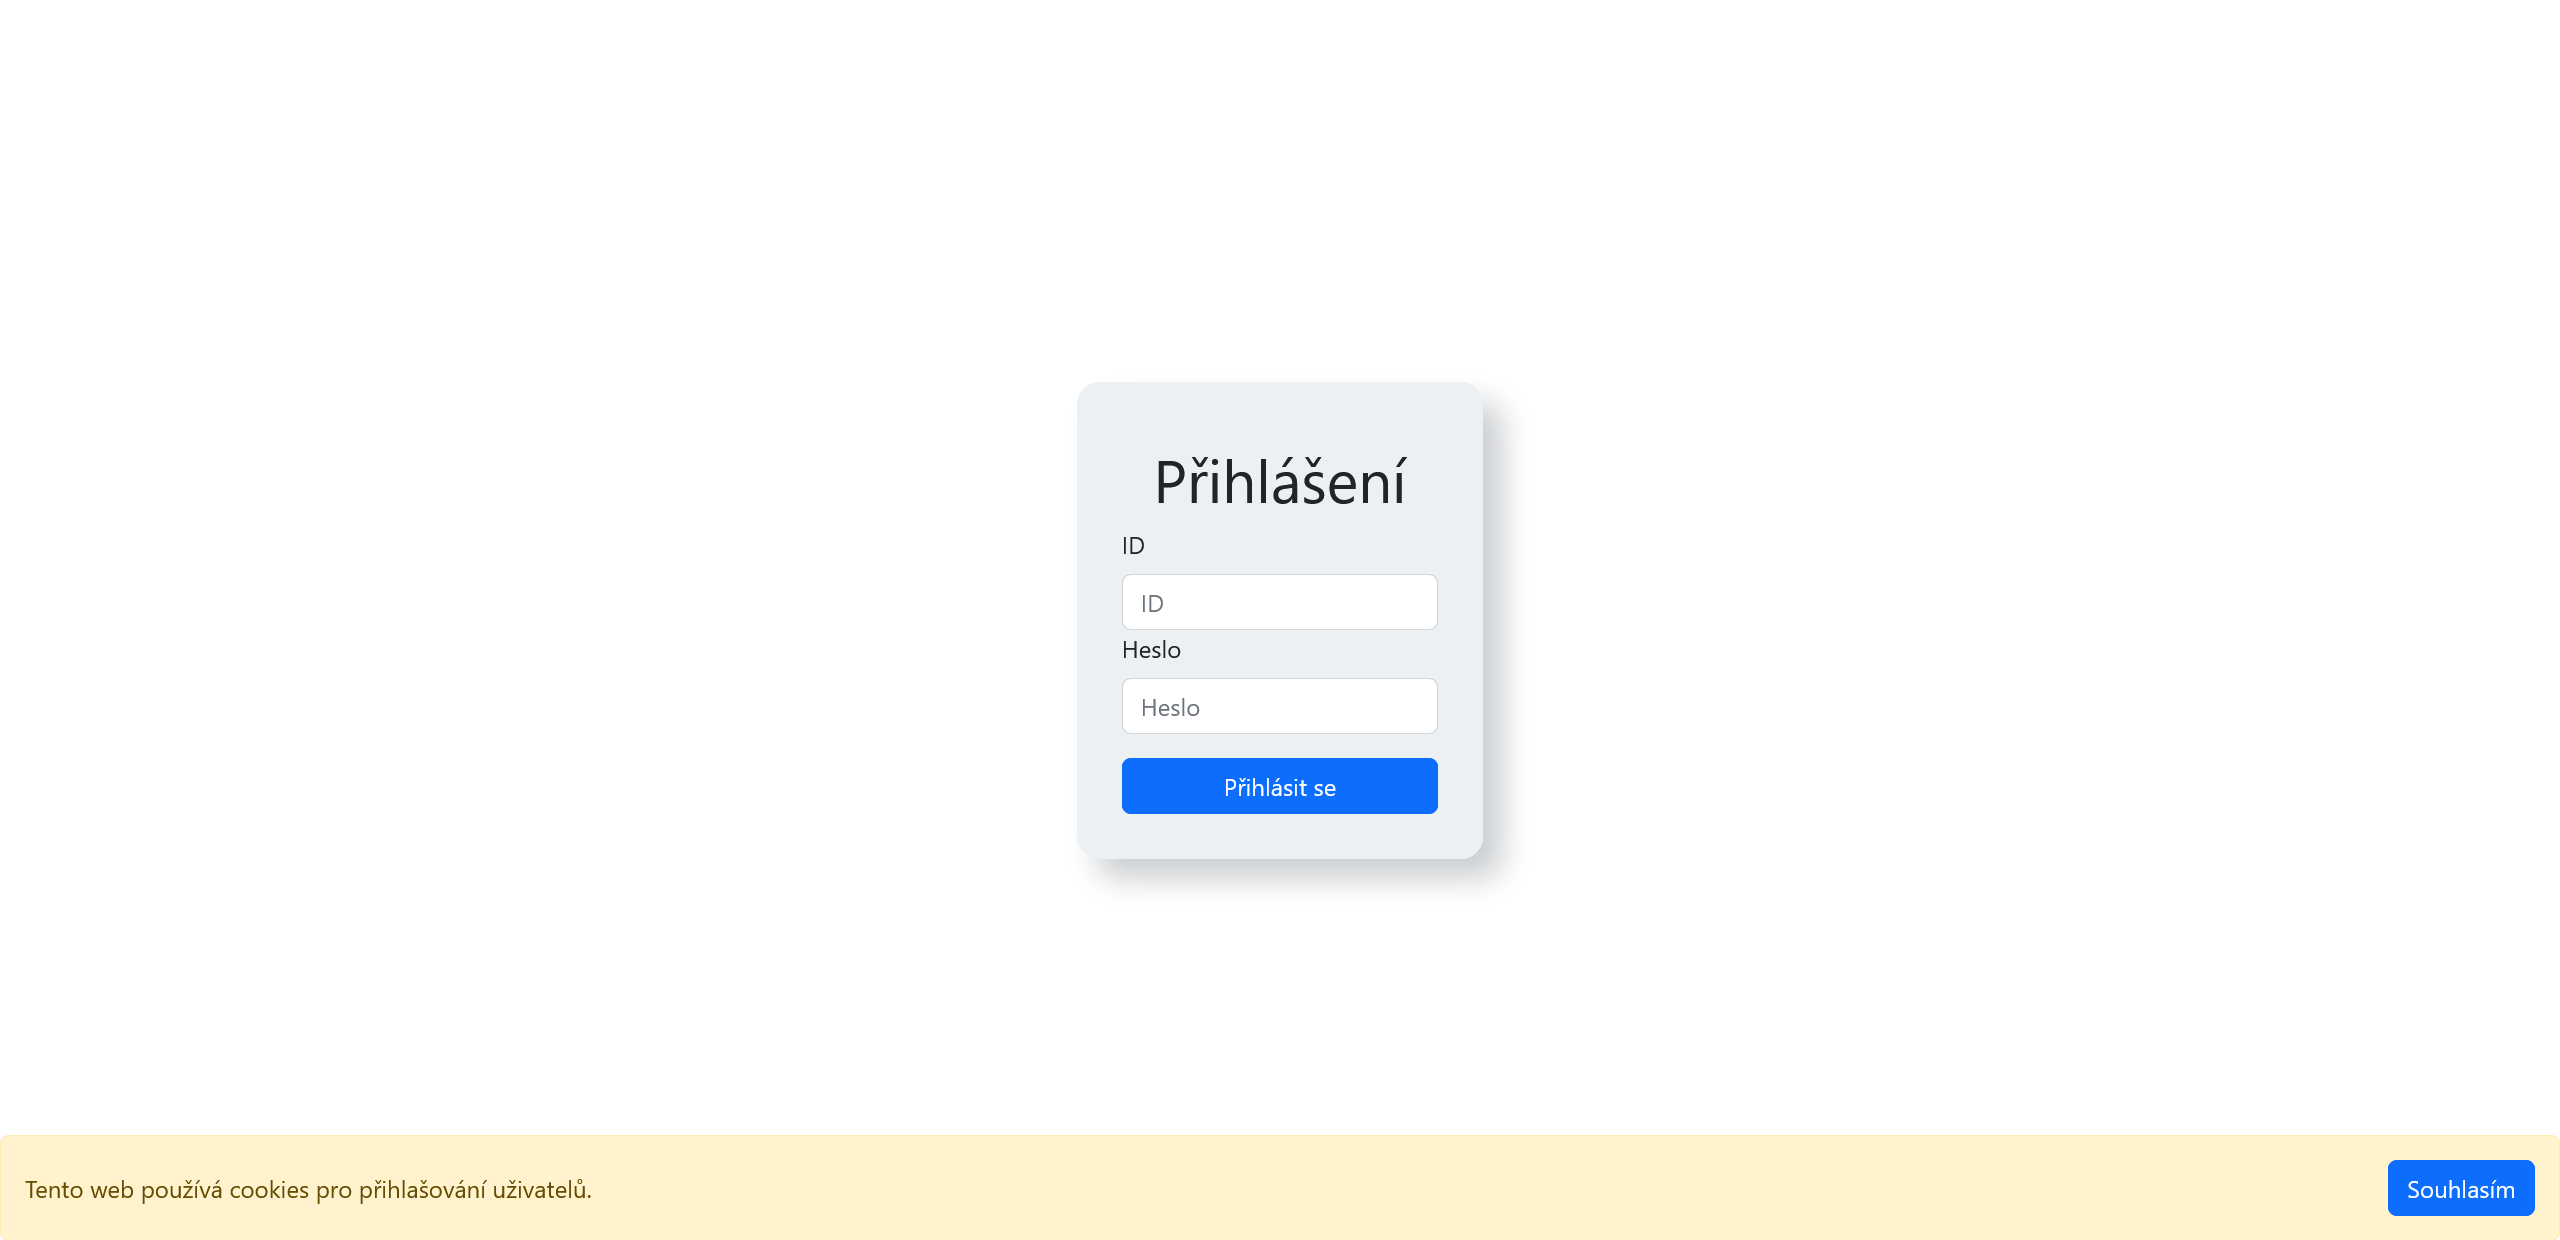
\includegraphics[width=\textwidth]{../img/screenshots/login}
    \caption{Přihlašovací obrazovka}\label{fig:login-screenshot}
\end{figure}


\section{Užívání aplikace z pohledu zaměstnance}\label{sec:uzivani-aplikace-z-pohledu-zamestnance}

Tato sekce popisuje užívání aplikace z pohledu zaměstnance.
Jsou zde popsány veškeré funkce, které byly identifikovány jako požadavky na funkcionalitu dostupnou zaměstnanci v kapitole~\ref{ch:analyza-pozadavku}.
Předpokládáme, že zaměstnanec má již vytvořený účet a přihlásil se do aplikace, jak je popsáno v sekci~\ref{sec:prihlaseni}, která se věnuje přihlášení a tvorbě účtu.
Po přihlášení je zaměstnanec automaticky přesměrován na výchozí obrazovku pro zaměstnance (Obr.~\ref{fig:sprava-formularu-screenshot}).

\subsection{Správa formulářů}\label{subsec:sprava-formularu}

Pro zadání úkolu plniteli je nutno nejprve vytvořit formulář.
Formuláře se vytváří v sekci \uv{Správa formulářů} (Obr.~\ref{fig:sprava-formularu-screenshot}).
Právo na tvorbu formulářů mají pouze zaměstnanci s rolí \uv{Správce dotazníků}.
Formuláře se vytváří pomocí tlačítka \uv{Nový formulář}.
Stisknutí tohoto tlačítka se dostaneme na stránku pro tvorbu formuláře (Obr.~\ref{fig:tvorba-formulare-screenshot}).
Pro vytvoření je potřeba zadat název formuláře do pole Název a přidat jednotlivé otázky taháním prvků z levého panelu do prostoru pro tvorbu formuláře.
Pole Identifikátor a Cesta se vyplní automaticky při zadání názvu a obvykle není třeba je měnit.
Jak vypočítat odvozené hodnoty v rámci vyhodnocení formuláře je popsáno v podsekci~\ref{subsubsec:vypocet-odvozenych-hodnot}.
Detailní dokumentace k tvorbě formulářů je dostupná online v anglickém jazyce na \href{https://help.form.io/userguide/form-building}{tomto odkazu}.
Formulář uložíme do systému pomocí tlačítka \uv{Vytvořit formulář}.
Obrazovka pro správu formulářů (Obr.~\ref{fig:sprava-formularu-screenshot}) nám nabízí několik dalších funkcí.
Již existující formuláře můžeme upravovat pomocí tlačítka \uv{Upravit} nebo mazat pomocí tlačítka \uv{Smazat}.
Úpravy formulářů mohou ovlivnit již existující odevzdání formulářů a proto se doporučuje tuto funkci používat pouze pro drobné opravy.

\begin{figure}[H]
    \centering
    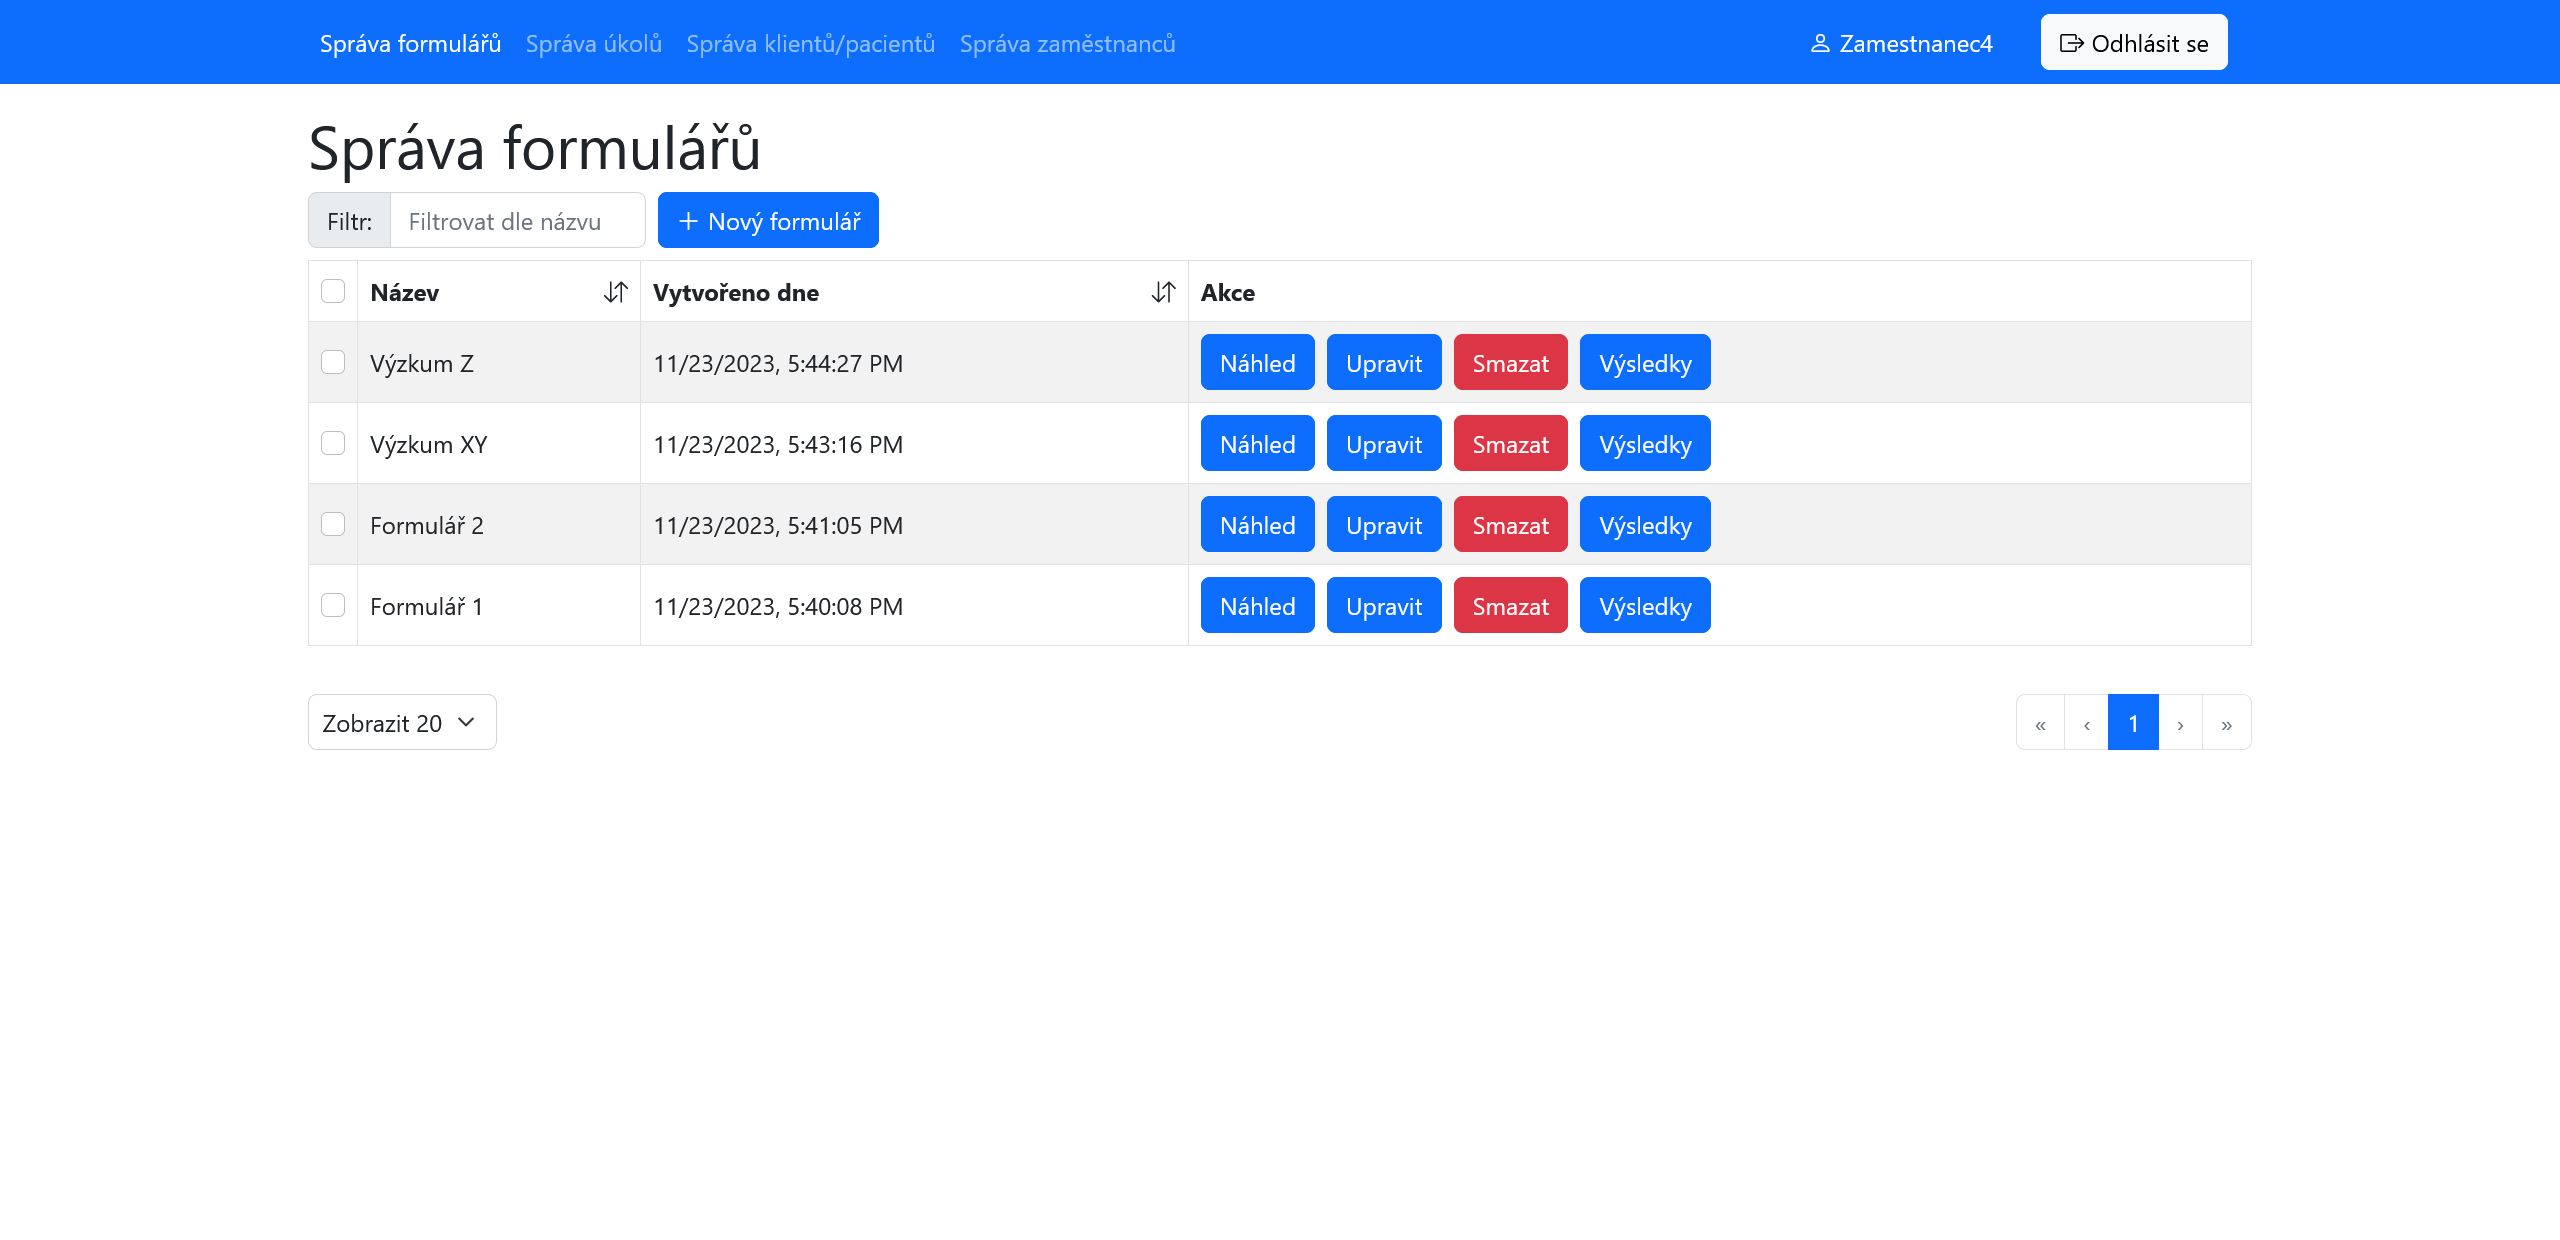
\includegraphics[width=\textwidth]{../img/screenshots/sprava-formularu}
    \caption{Správa formulářů aplikace}\label{fig:sprava-formularu-screenshot}
\end{figure}

\begin{figure}[H]
    \centering
    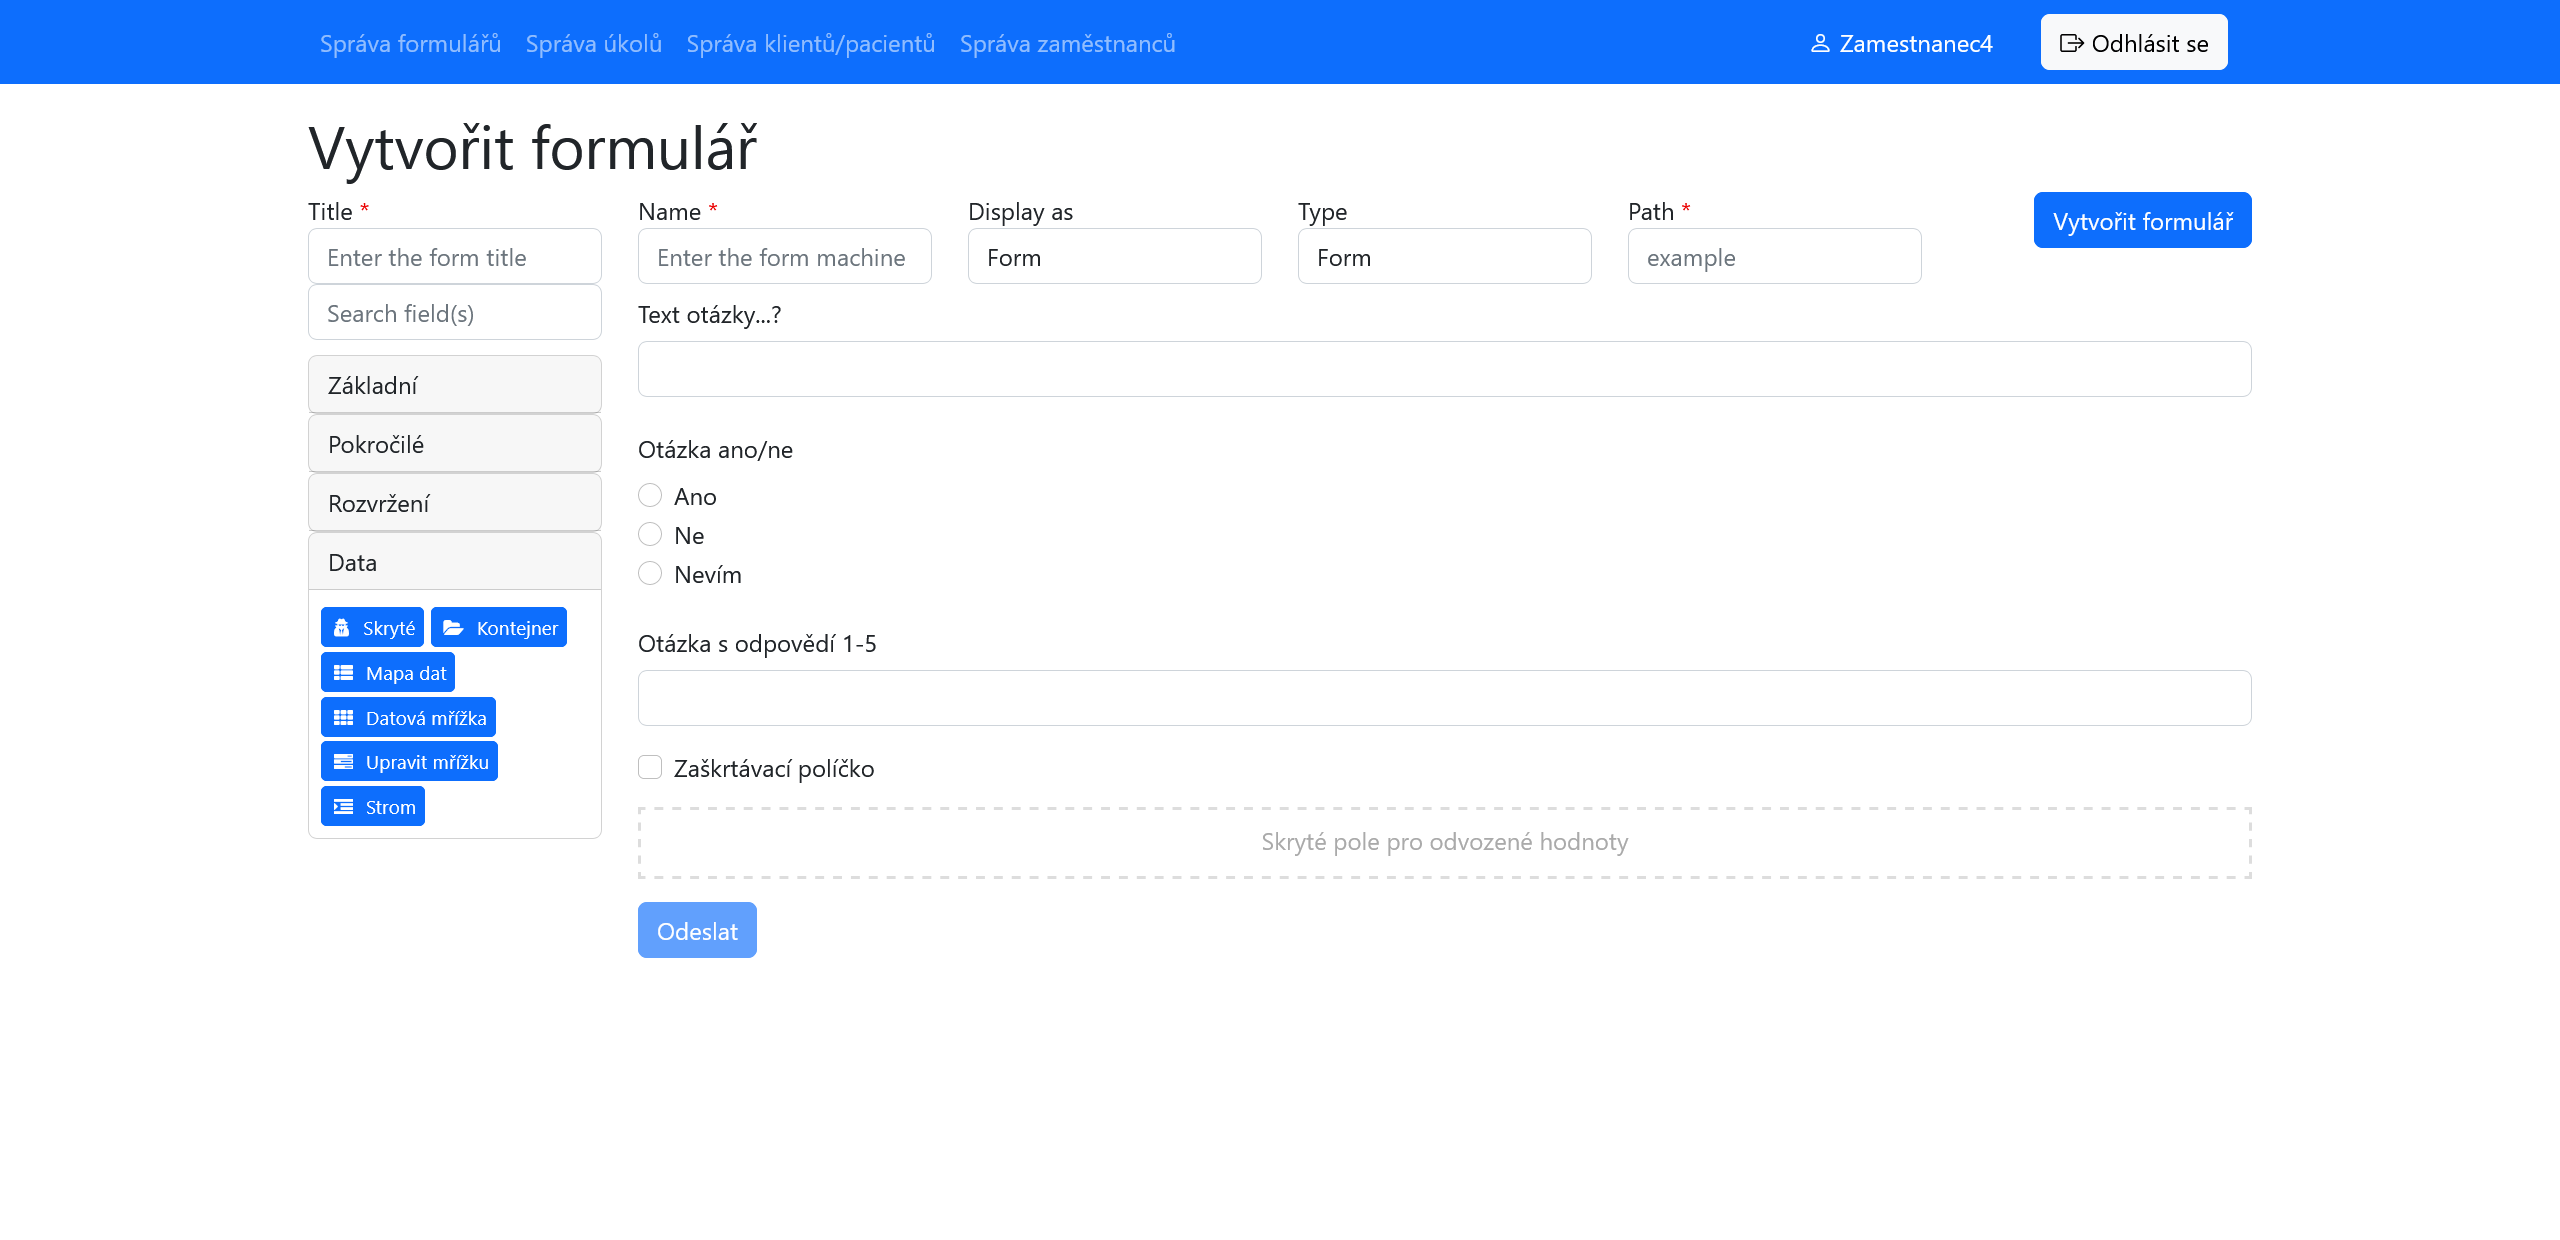
\includegraphics[width=\textwidth]{../img/screenshots/tvorba-formulare}
    \caption{Správa formulářů aplikace}\label{fig:tvorba-formulare-screenshot}
\end{figure}

\subsubsection{Výpočet odvozených hodnot}\label{subsubsec:vypocet-odvozenych-hodnot}

Pokud chceme formulář automaticky vyhodnotit na základě odpovědí plnitele, použijeme prvek \uv{Skryté} z kategorie \uv{Data} z levého panelu.
Po přidání prvku se zobrazí jeho nastavení (Obr.~\ref{fig:odvozena-hodnota-nastaveni}).
Vzorec pro výpočet hodnoty můžeme zadat do sekce \uv{Vypočtená hodnota} v kartě \uv{Data} (Obr.~\ref{fig:odvozena-hodnota-vzorec-a-server}).
Vzorec se zapisuje v programovacím jazyce \href{https://developer.mozilla.org/en-US/docs/Web/JavaScript}{JavaScript}.
Všechny hodnoty odpovědí jsou dostupné na objektu \lstinline{data}.
Vzorec používá názvy vlastností jako klíče na tomto objektu.
Pro použití konkrétní můžeme použít tečkovou notaci \lstinline{data.nazevVlastnosti} nebo notaci s hranatými závorkami \lstinline{data["nazevVlastnosti"]}.
Název vlastnosti lze pro každý prvek nastavit v menu nastavení v poli \uv{Název vlastnosti} v kartě \uv{API} (Obr.~\ref{fig:odvozena-hodnota-nastaveni-nazev}).
Výsledek vzorce uložíme do proměnné \lstinline{value}.
Např.\ pro součet hodnoty odpovědí s názvy \uv{a} a \uv{b} bychom použili vzorec \lstinline{value = data.a + data.b}.
Pokud je nevhodné, aby uživatel viděl způsob výpočtu odvozené hodnoty nebo mohl získat vypočtenou hodnotu, tak je nutné v nastavení prvku zvolit možnost \uv{Vypočítat hodnotu na serveru} (Obr.~\ref{fig:odvozena-hodnota-vzorec-a-server}).
Nastavení prvku uložíme stisknutím tlačítka \uv{Uložit}.
Kdybychom chtěli nastavení prvku znovu upravit, tak se na obrazovku nastavení dostaneme stisknutím tlačítka s ozubeným kolečkem v pravém horním rohu prvku (Obr.~\ref{fig:odvozena-hodnota-ozubene-kolo}).

\begin{figure}[H]
    \centering
    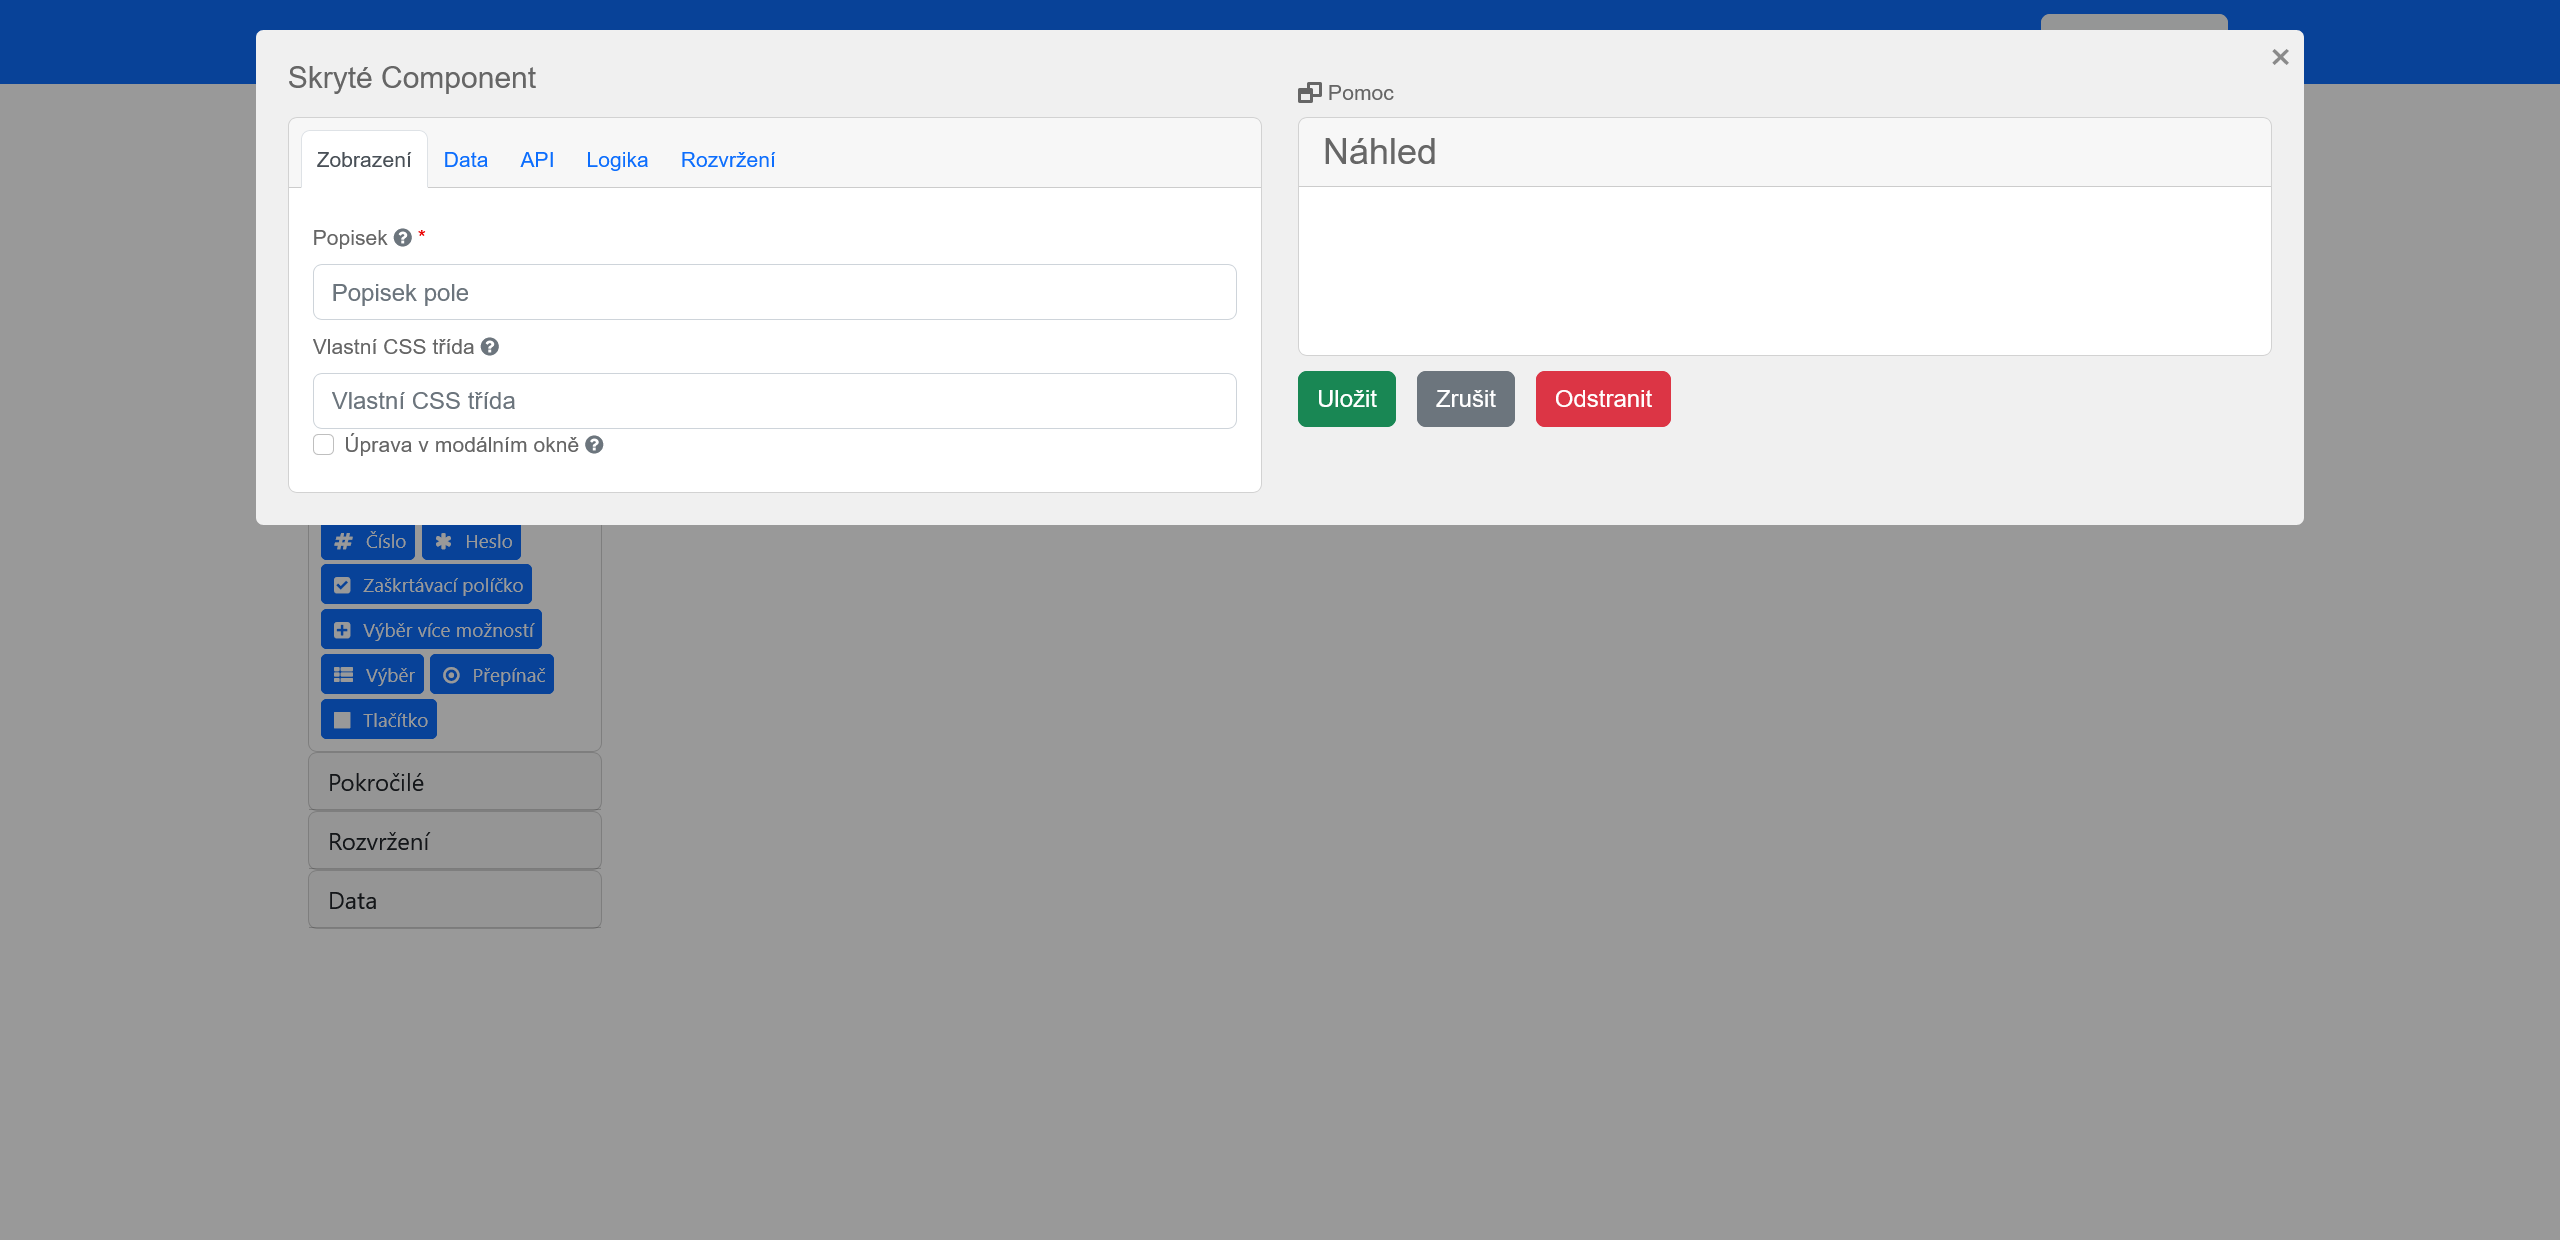
\includegraphics[width=\textwidth]{../img/screenshots/odvozena-hodnota-nastaveni}
    \caption{Karta Zobrazení v nastavení prvku Skryté}\label{fig:odvozena-hodnota-nastaveni}
\end{figure}

\begin{figure}[H]
    \centering
    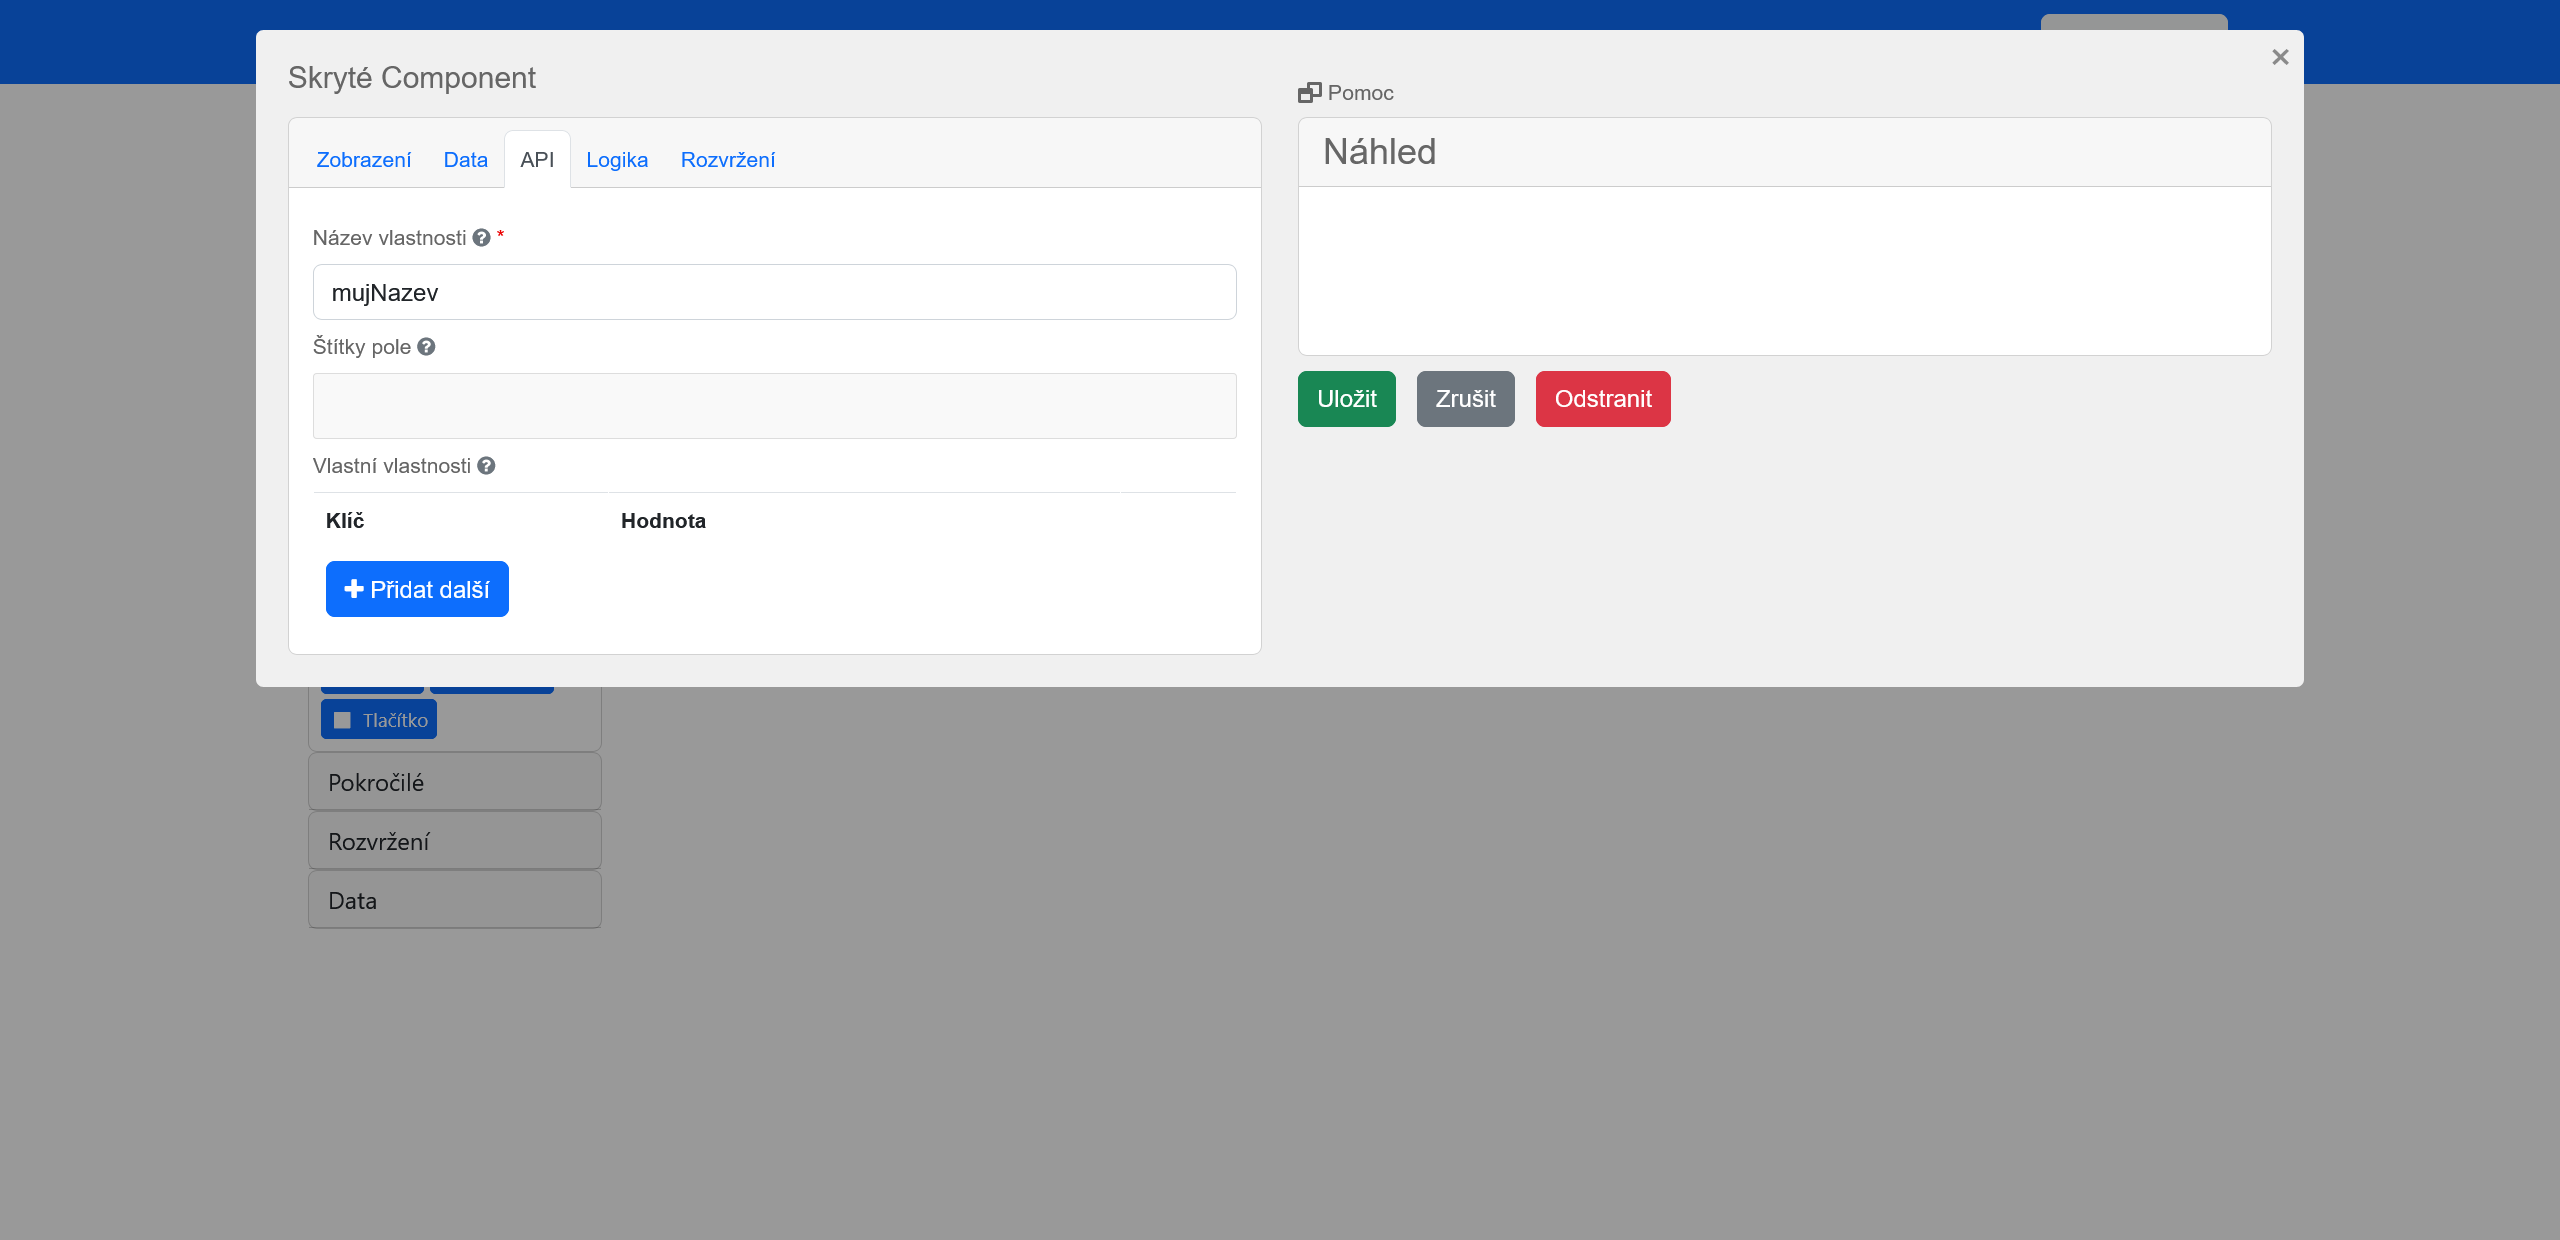
\includegraphics[width=\textwidth]{../img/screenshots/odvozena-hodnota-nastaveni-nazvu}
    \caption{Karta API v nastavení prvku Skryté}\label{fig:odvozena-hodnota-nastaveni-nazev}
\end{figure}

\begin{figure}[H]
    \centering
    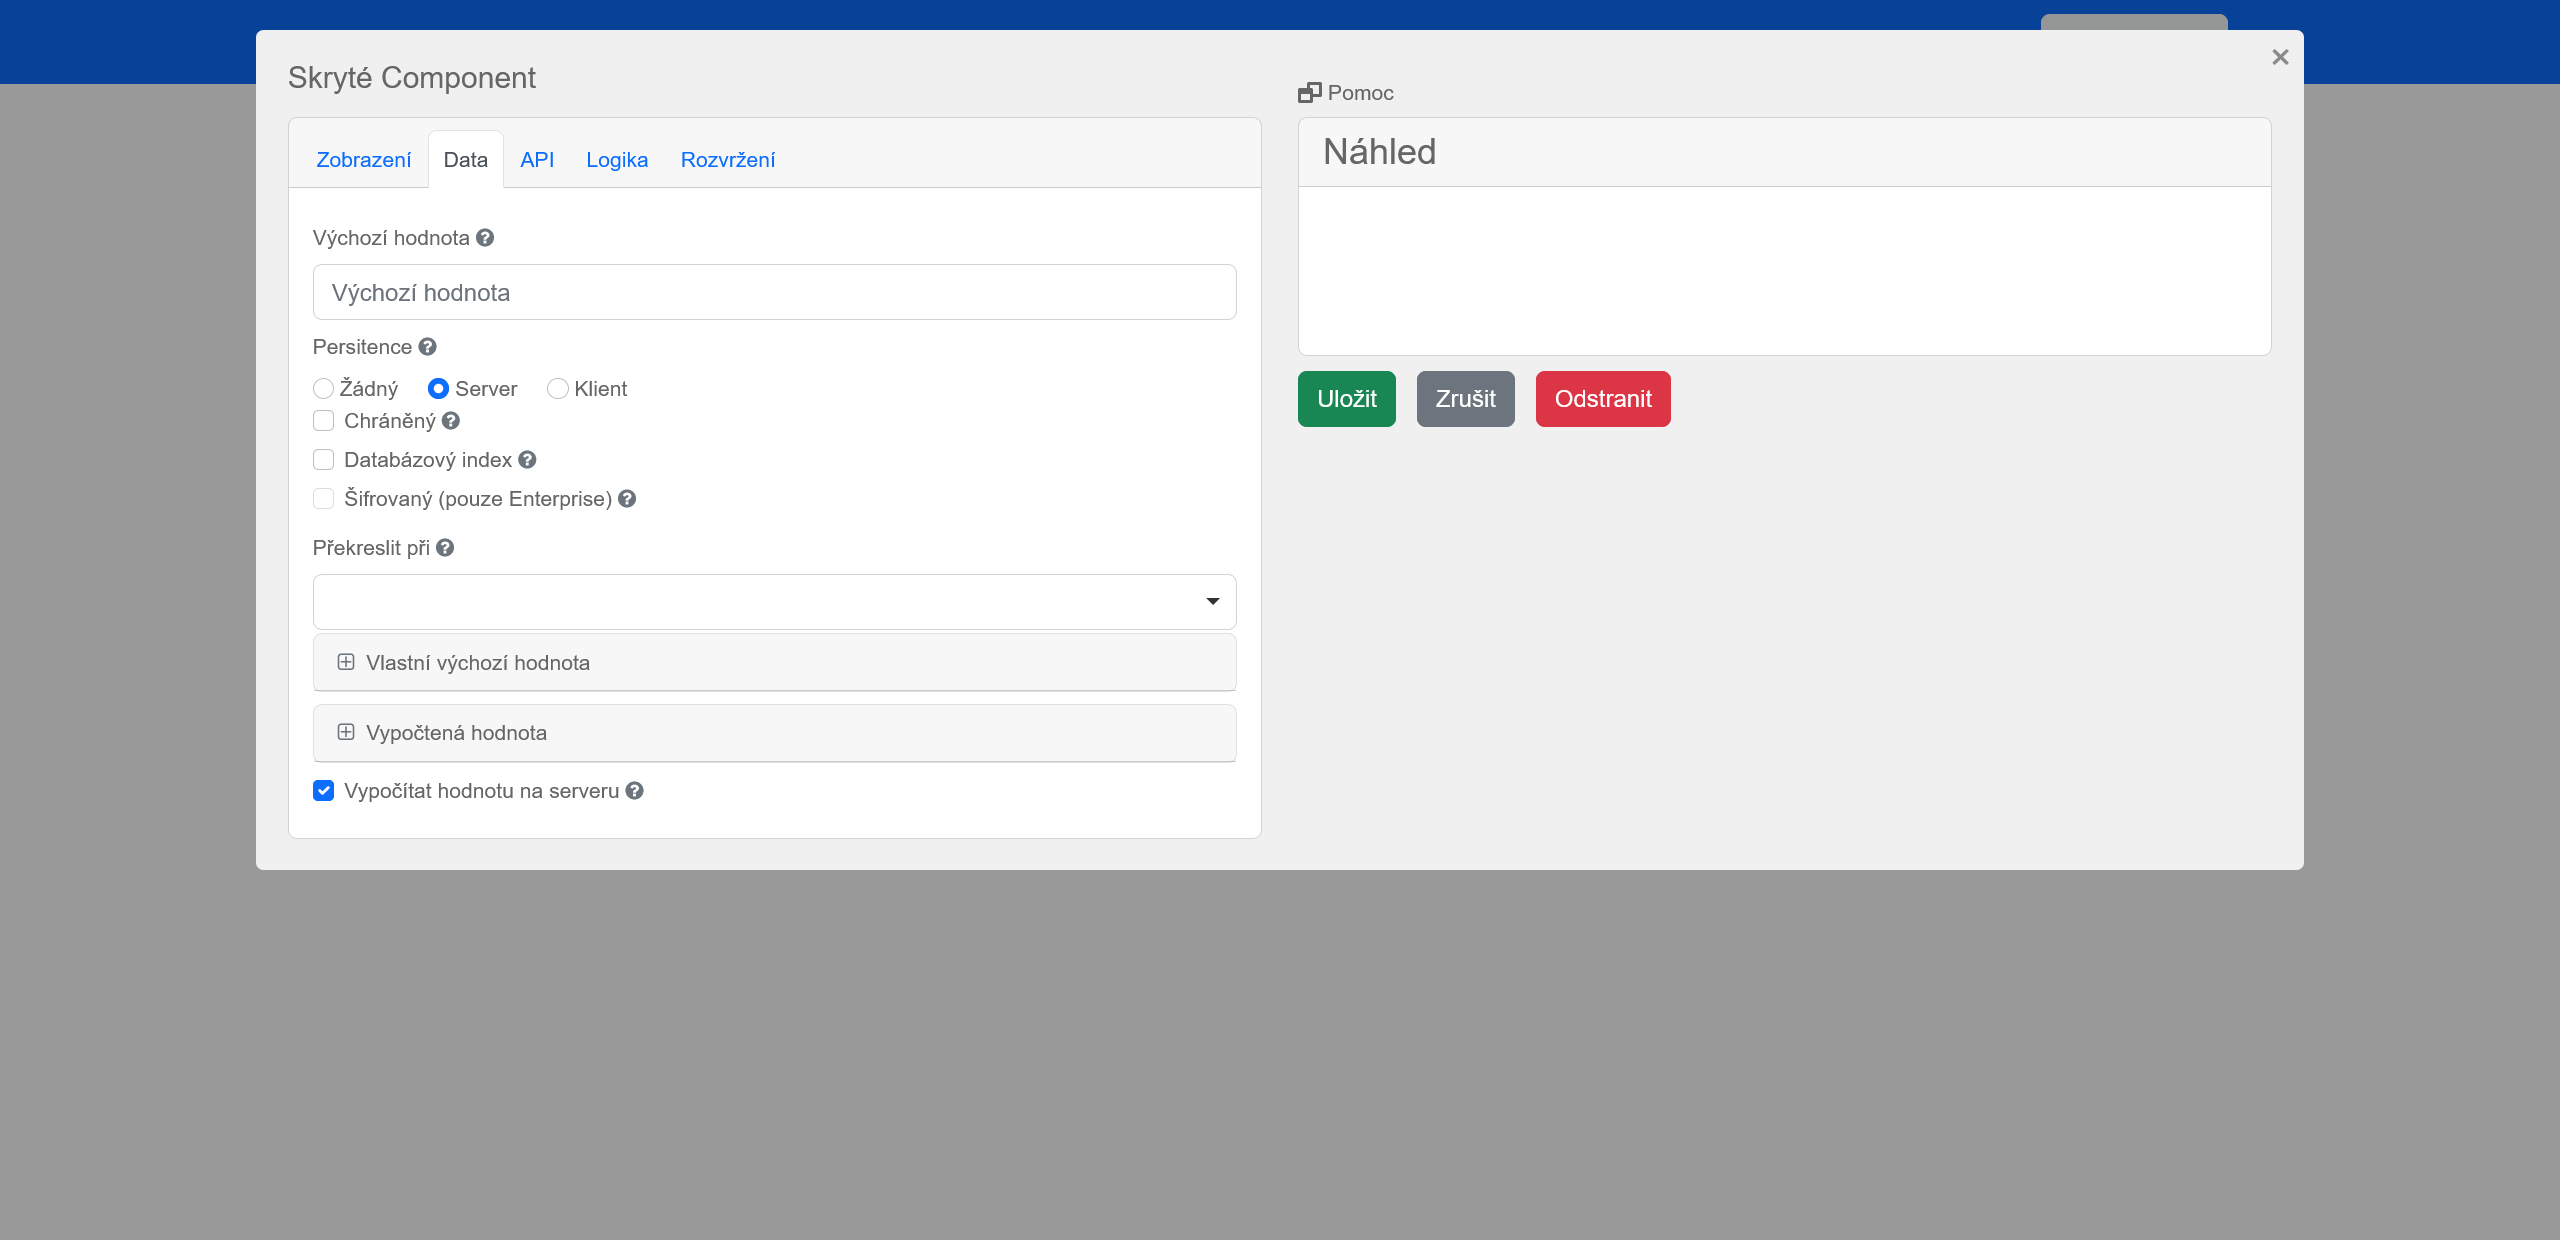
\includegraphics[width=\textwidth]{../img/screenshots/odvozena-hodnota-vzorec-a-server}
    \caption{Karta Data v nastavení prvku Skryté}\label{fig:odvozena-hodnota-vzorec-a-server}
\end{figure}

\begin{figure}[H]
    \centering
    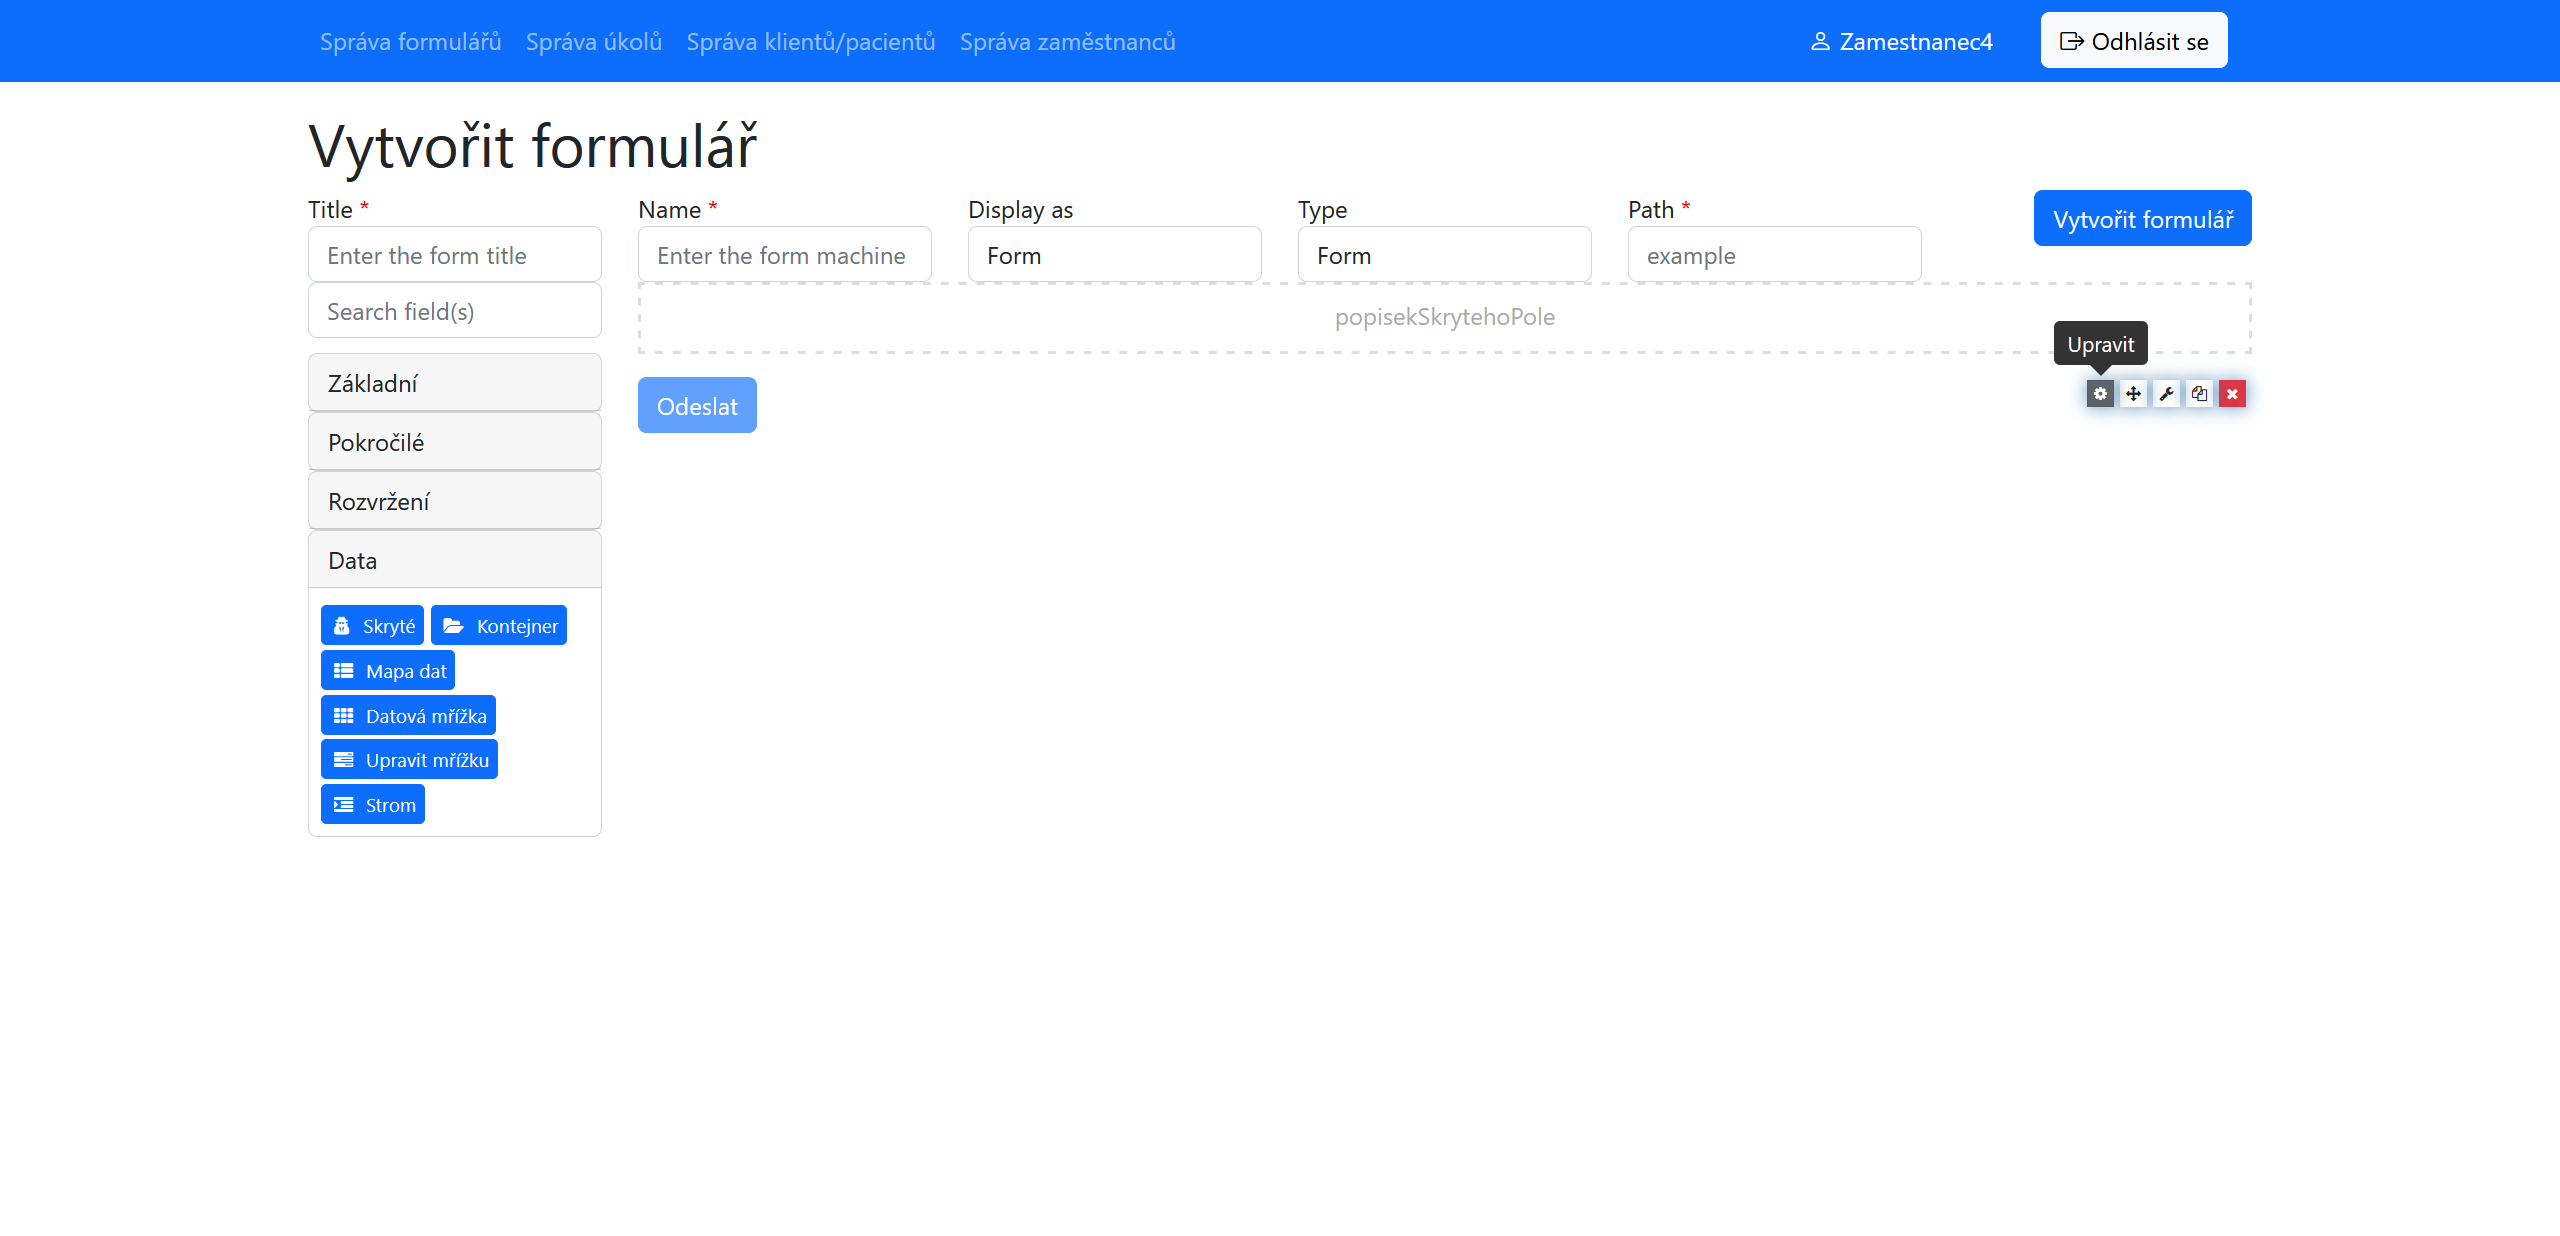
\includegraphics[width=\textwidth]{../img/screenshots/odvozena-hodnota-ozubene-kolo}
    \caption{Zobrazení menu nastavení prvku}\label{fig:odvozena-hodnota-ozubene-kolo}
\end{figure}

\subsection{Správa plnitelů}\label{subsec:sprava-plnitelu}

Pro zadání úkolu plniteli je nutno nejprve vytvořit uživatelský účet pro plnitele.
Účty plnitelů se vytváří v sekci \uv{Správa plnitelů} (Obr.~\ref{fig:sprava-plnitelu-screenshot}).
Nový účet vytvoříme pomocí tlačítka \uv{Založit účet nového klienta/pacienta}.
Pro vytvoření účtu je potřeba zadat identifikátor plnitele, který je unikátní v rámci celé aplikace, a heslo.
Plnitel si může heslo změnit po přihlášení do aplikace.

\begin{figure}[H]
    \centering
    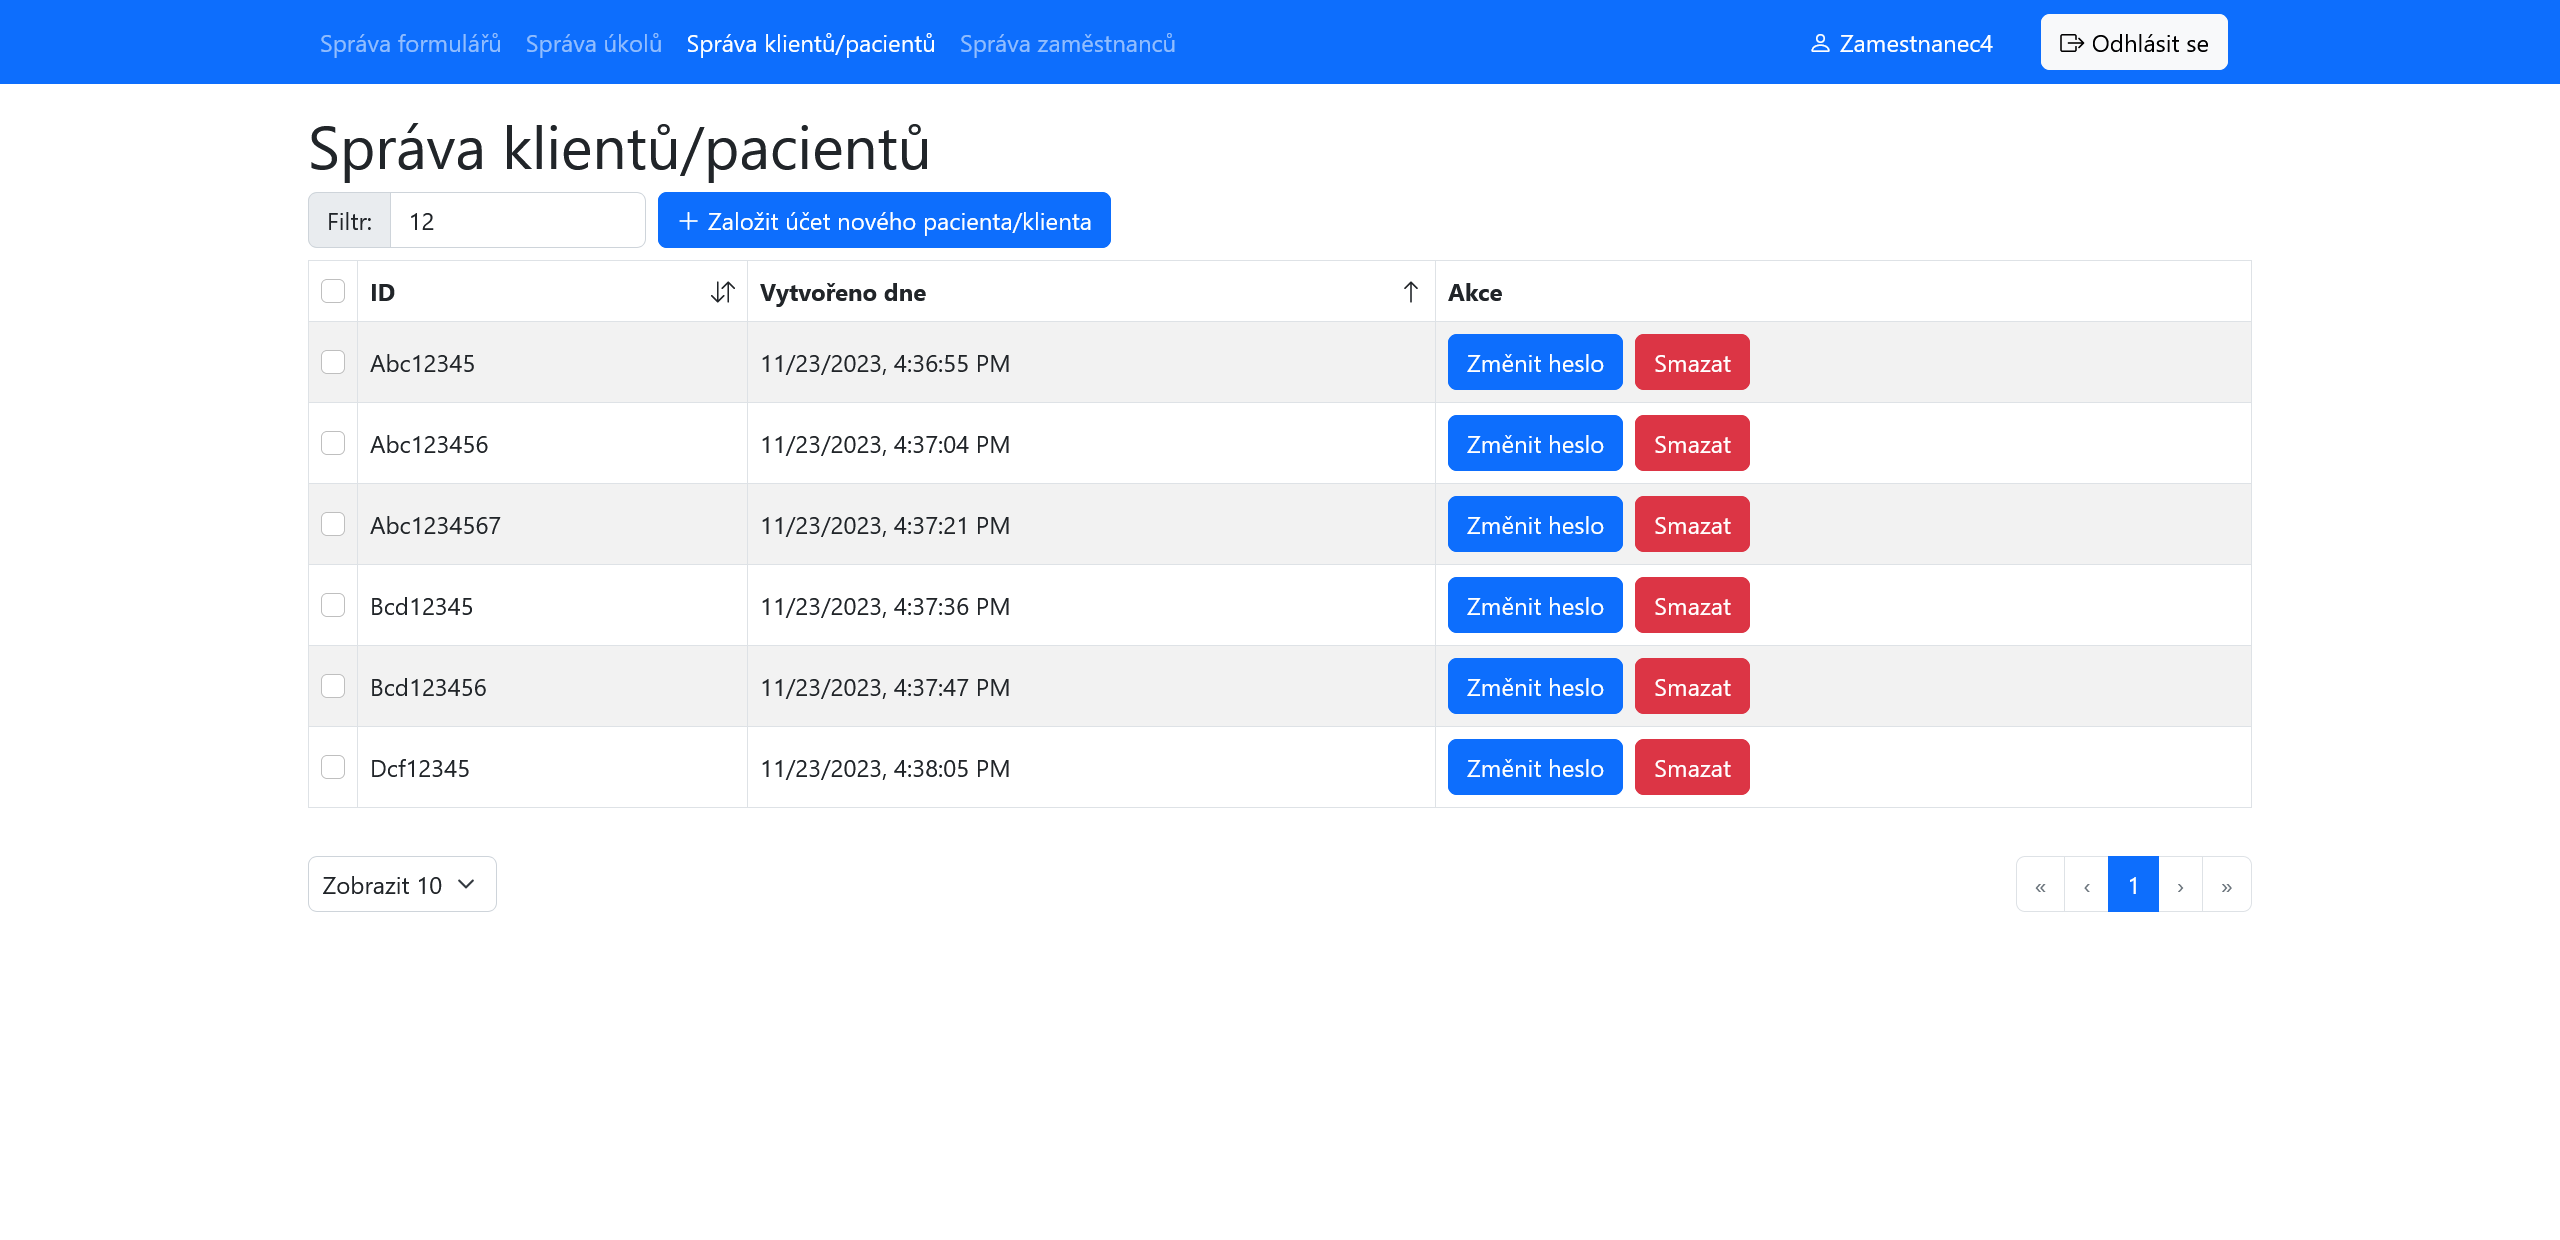
\includegraphics[width=\textwidth]{../img/screenshots/sprava-plnitelu}
    \caption{Správa účtů plnitelů}\label{fig:sprava-plnitelu-screenshot}
\end{figure}

\subsection{Správa úkolů}\label{subsec:sprava-ukolu}

Nyní můžeme vytvořit úkol pro plnitele.
Úkoly se vytváří v sekci \uv{Správa úkolů} (Obr.~\ref{fig:sprava-ukolu-screenshot}).
Nový úkol vytvoříme pomocí tlačítka \uv{Nový úkol}.
Stisknutím tohoto tlačítka se dostaneme na stránku pro tvorbu úkolu (Obr.~\ref{fig:tvorba-ukolu-screenshot}).
Pro vytvoření je potřeba zadat název úkolu, vybrat formulář, který má plnitel vyplnit, a vybrat plnitele.
Při tvorbě je možno zvolit více plnitelů a tím zadat více úkolů najednou.
K úkolu můžeme volitelně přidat popis, start, deadline a opakování.
Start úkolu je datum a čas, od kdy je možné úkol splnit.
Deadline úkolu je datum a čas, do kdy je možné úkol splnit.
Start a deadline byly takto definovány v kapitole~\ref{ch:analyza-pozadavku}.
Můžeme povolit překročení deadline, ale standardně je po deadline úkol uzavřen a nelze jej splnit.
Obrazovka pro konfiguraci deadline je zobrazena na obrázku~\ref{fig:tvorba-ukolu-deadline-screenshot}.
Při nastavení opakování je vytvořeno více úkolu najednou pro jednoho uživatele.
Pokud chceme vytvořit opakující se úkol, tak je nutné také definovat deadline, který je vždy posunut o interval specifikovaný v nastavení opakování.
Obrazovka pro konfiguraci opakování je zobrazena na obrázku~\ref{fig:tvorba-ukolu-opakovani-screenshot}.

\begin{figure}[H]
    \centering
    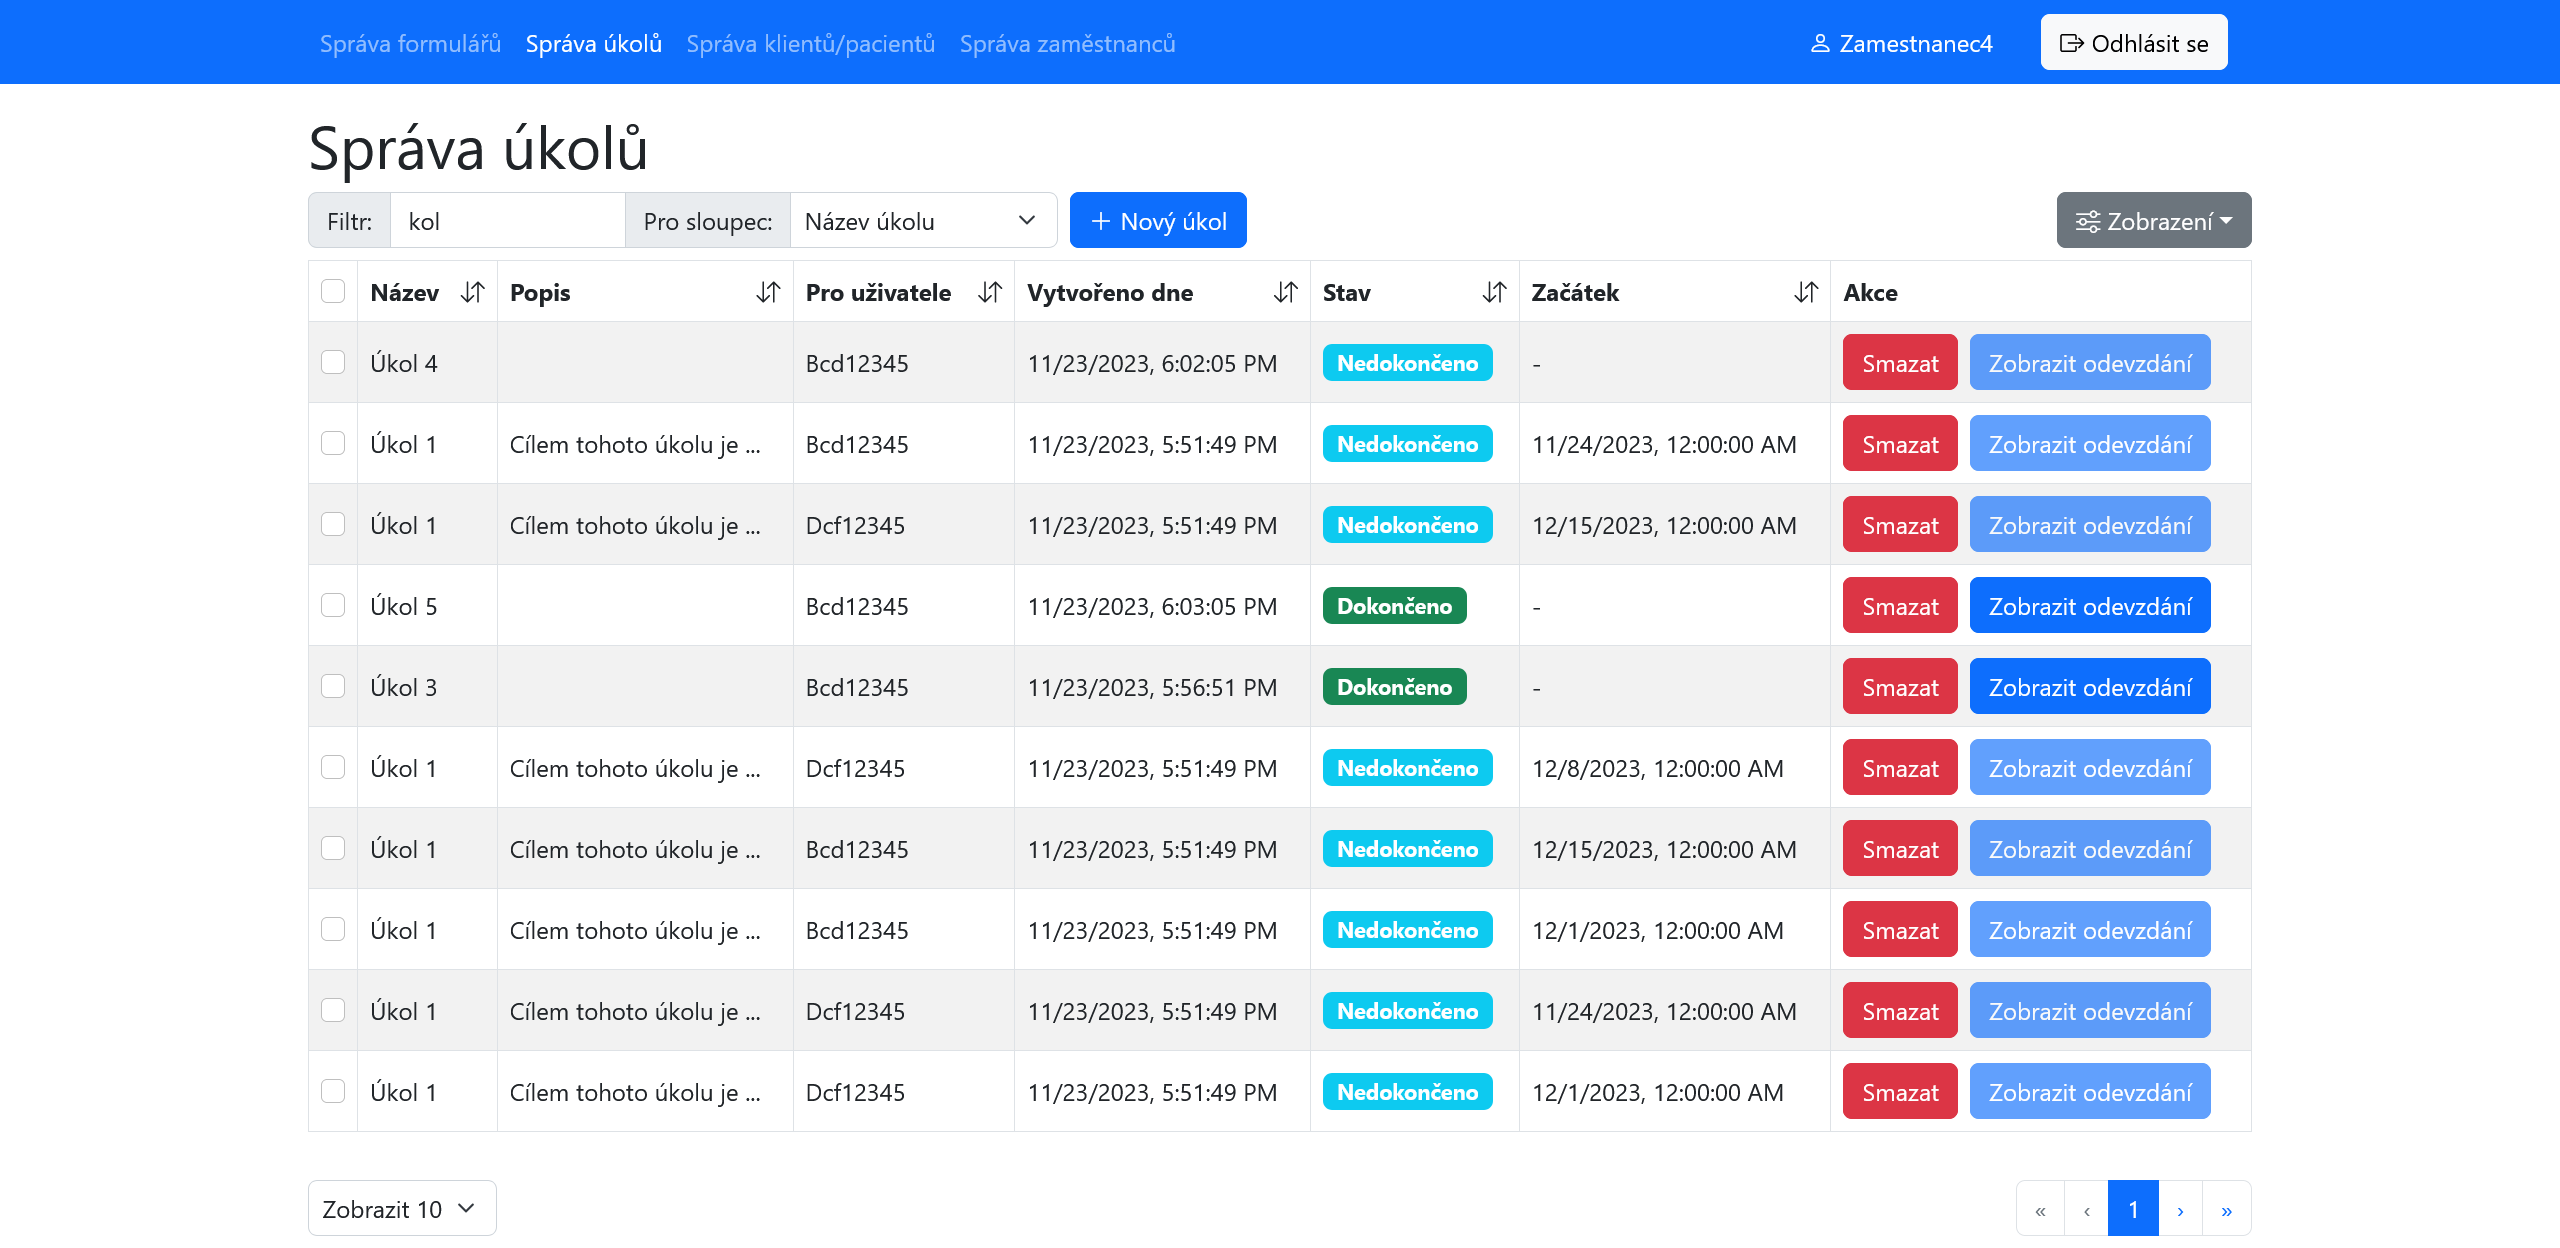
\includegraphics[width=\textwidth]{../img/screenshots/sprava-ukolu}
    \caption{Správa úkolů}\label{fig:sprava-ukolu-screenshot}
\end{figure}

\begin{figure}[H]
    \centering
    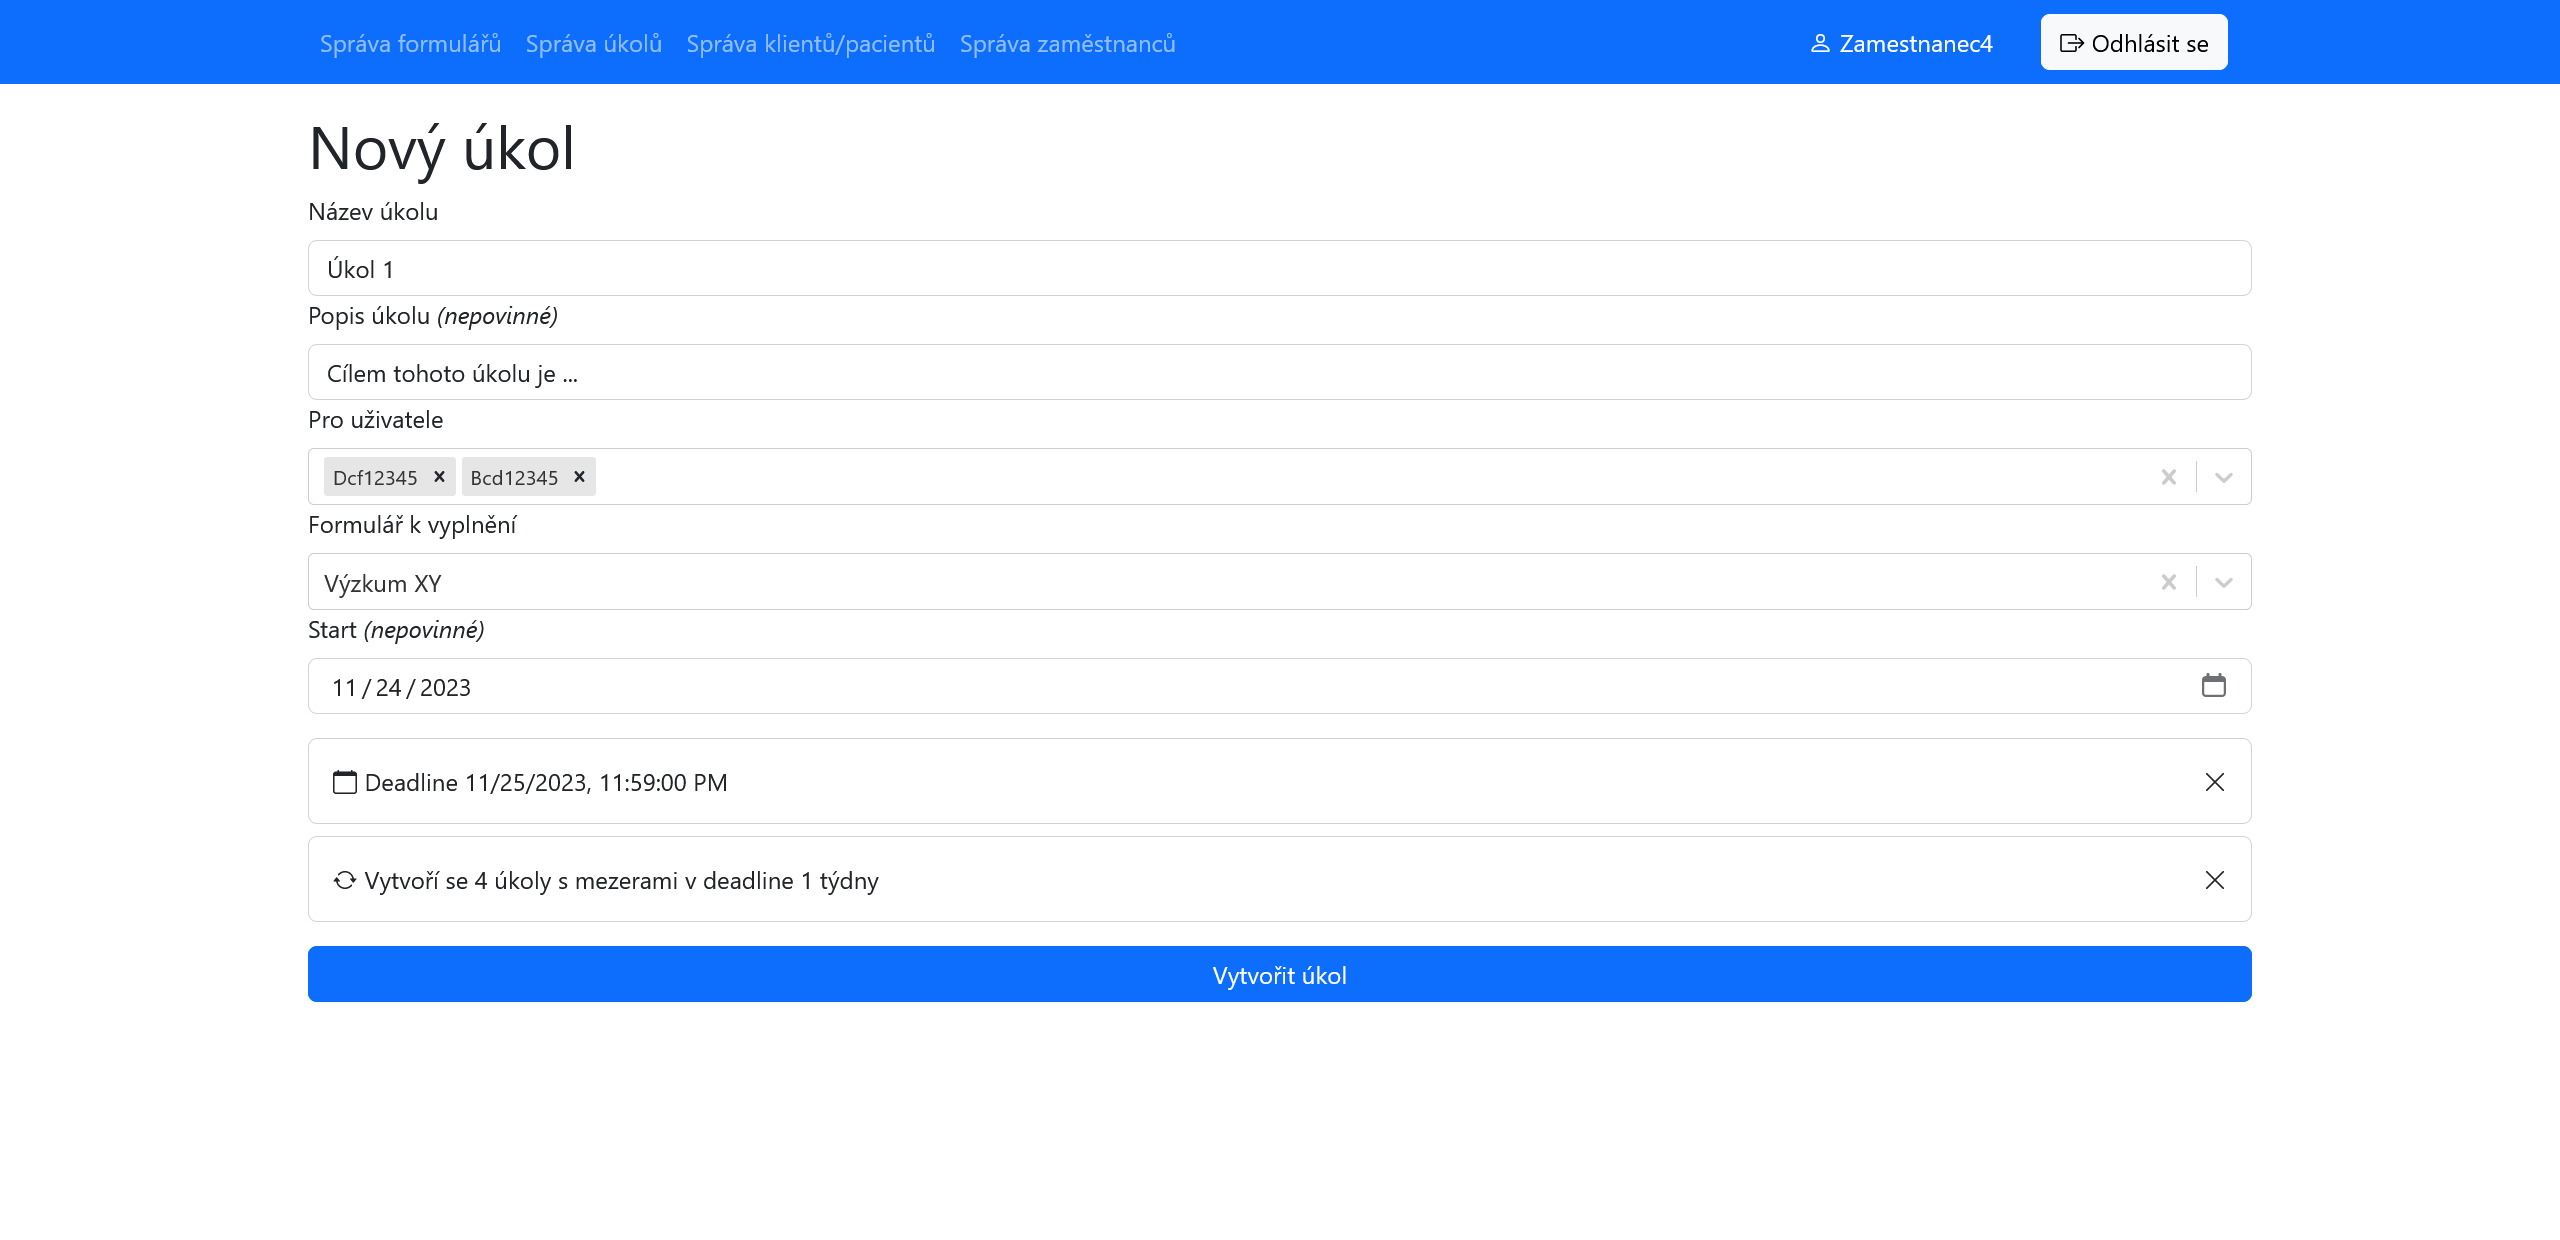
\includegraphics[width=\textwidth]{../img/screenshots/tvorba-ukolu}
    \caption{Tvorba úkolu}\label{fig:tvorba-ukolu-screenshot}
\end{figure}

\begin{figure}[H]
    \centering
    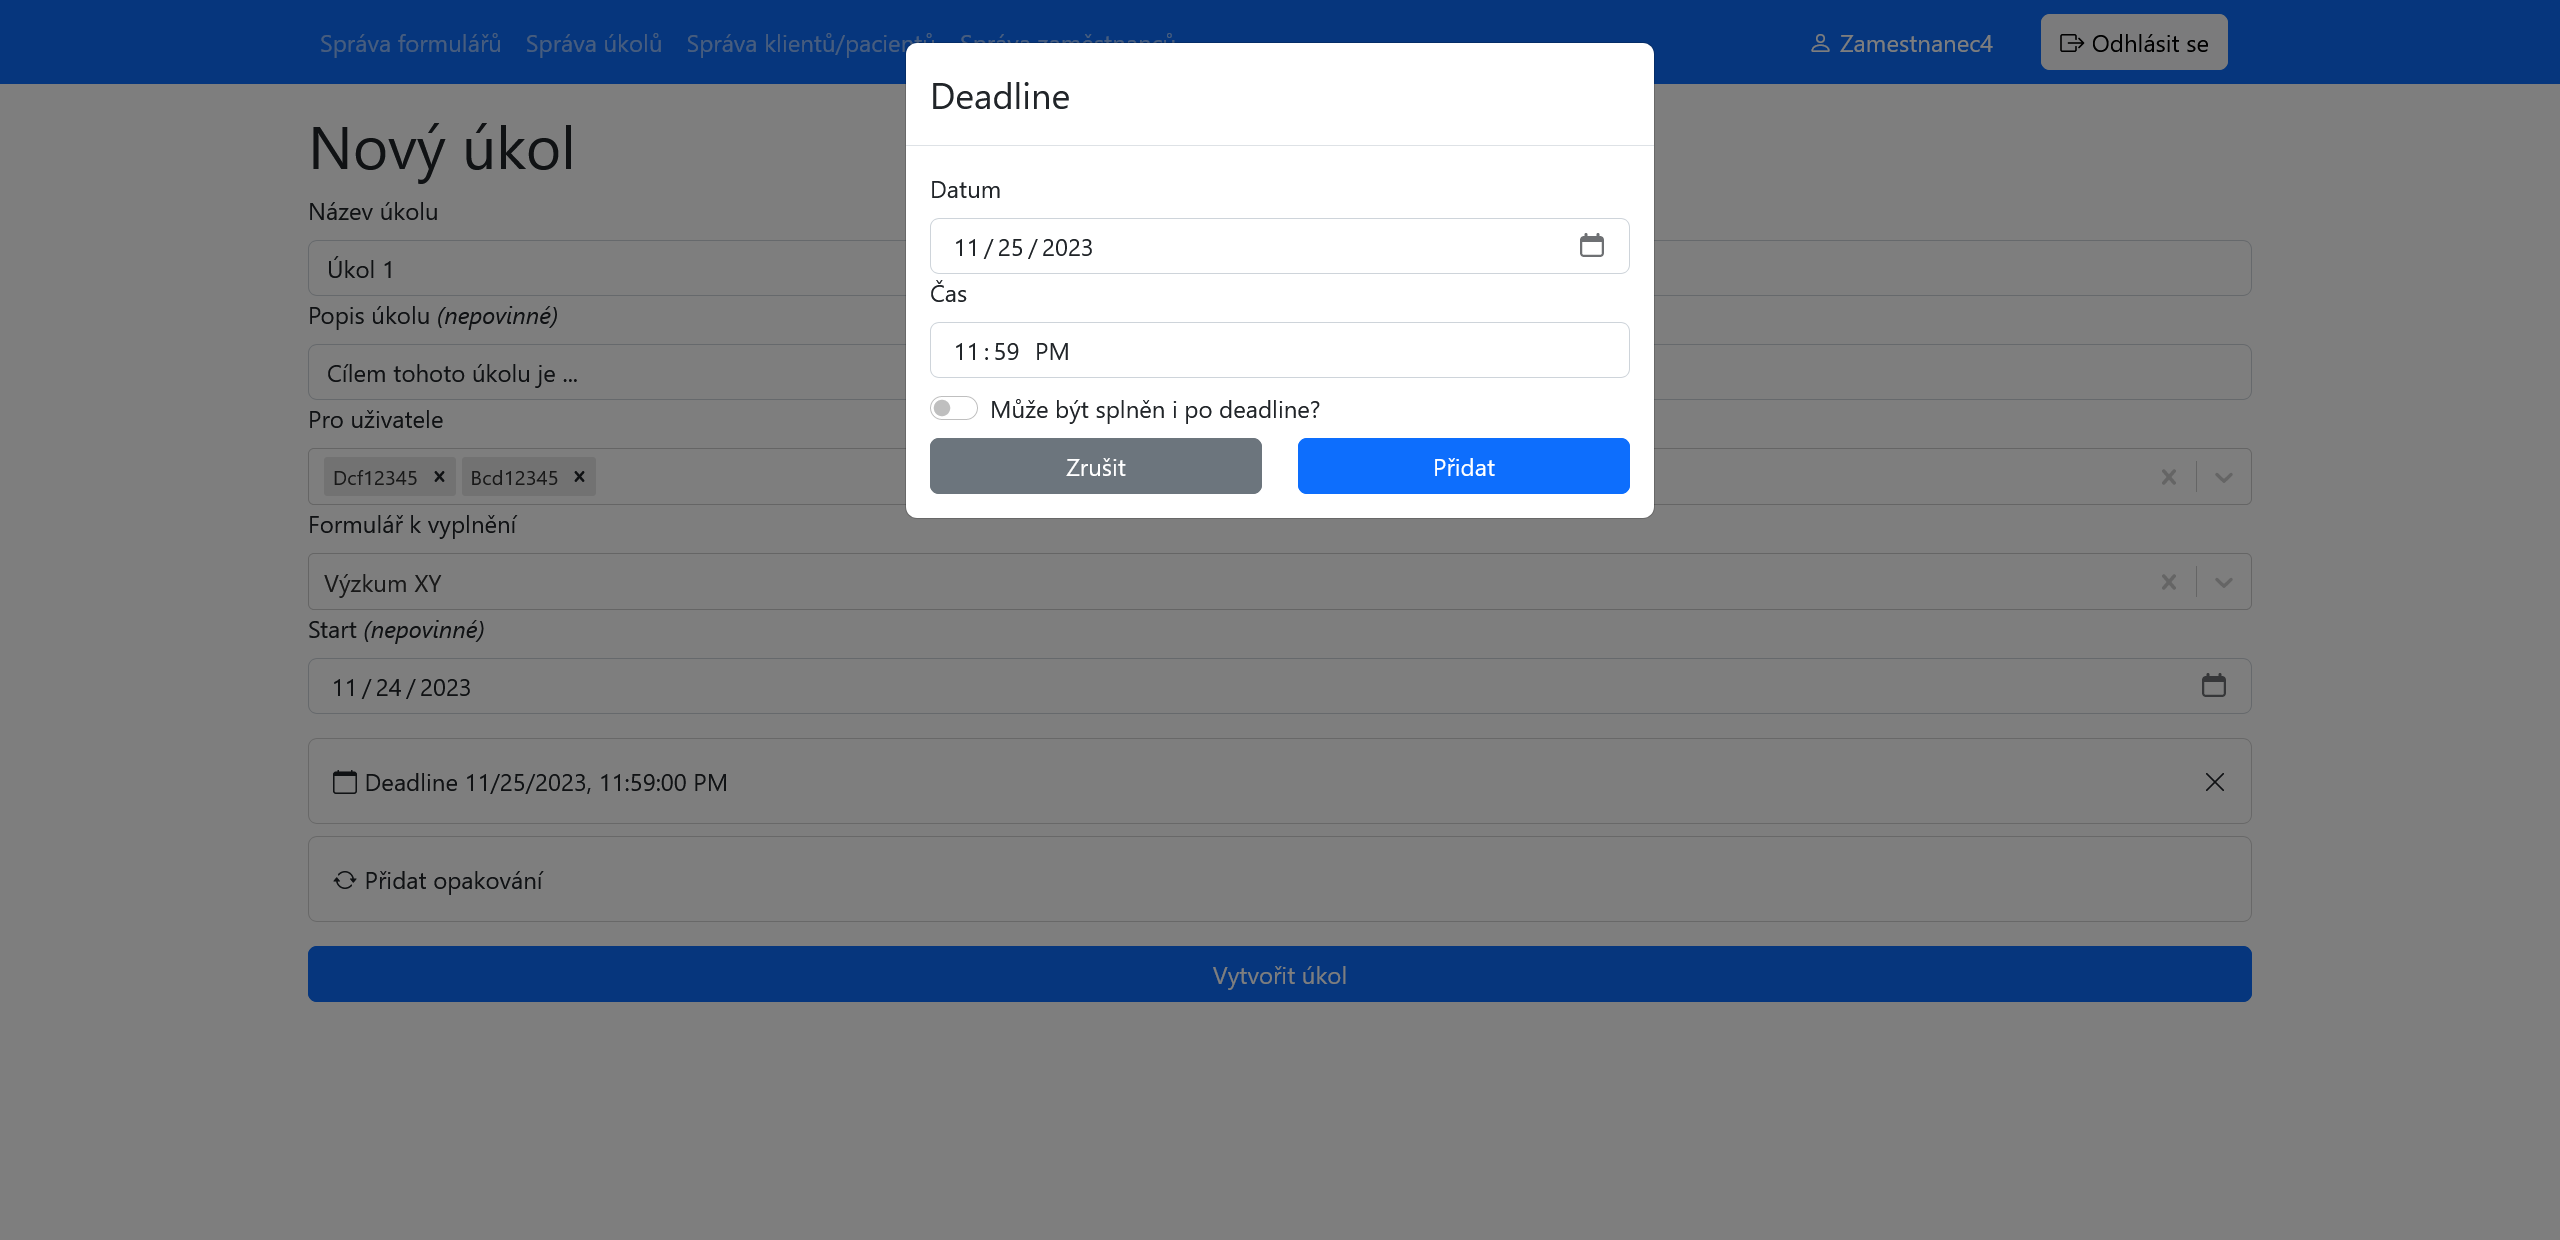
\includegraphics[width=\textwidth]{../img/screenshots/tvorba-ukolu-deadline}
    \caption{Zadávání deadline při tvorbě úkolu}\label{fig:tvorba-ukolu-deadline-screenshot}
\end{figure}

\begin{figure}[H]
    \centering
    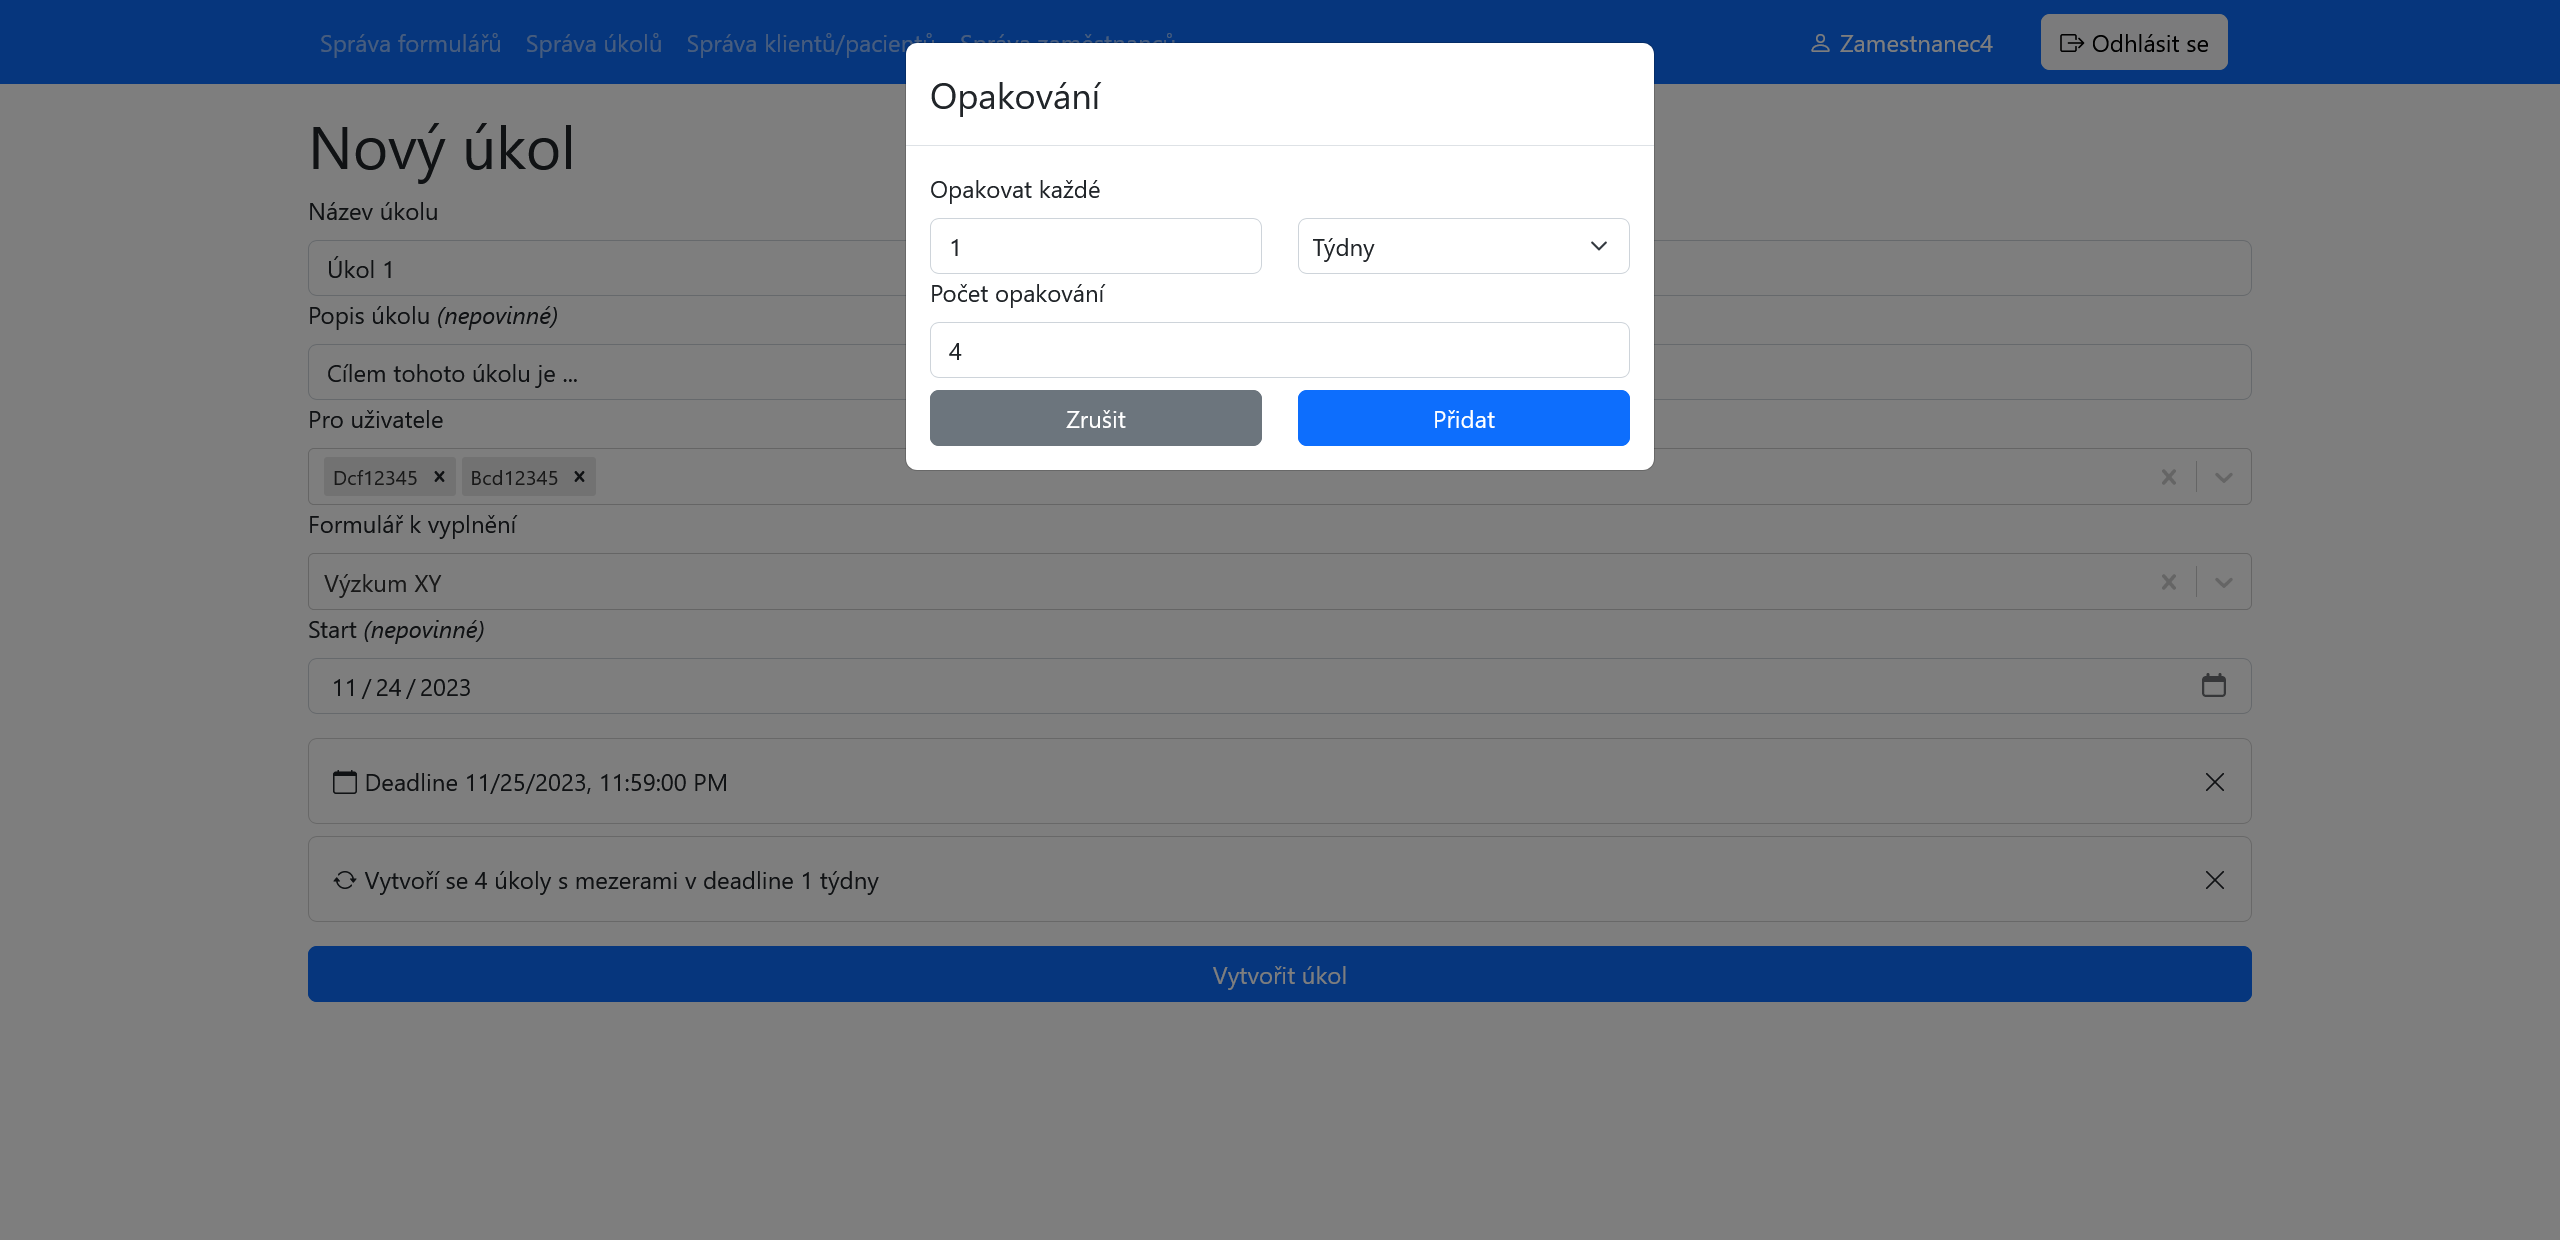
\includegraphics[width=\textwidth]{../img/screenshots/tvorba-ukolu-opakovani}
    \caption{Konfigurace opakování při tvorbě úkolu}\label{fig:tvorba-ukolu-opakovani-screenshot}
\end{figure}

\subsection{Náhled na odevzdání formuláře}\label{subsec:nahled-odevzdani-formulare}

Nyní předpokládejme, že plnitel splnil zadaný úkol.
Zaměstnanec si může zobrazit odevzdání formuláře pomocí tlačítka \uv{Zobrazit odevzdání} v sekci \uv{Správa úkolů} (Obr.~\ref{fig:sprava-ukolu-screenshot}).
Náhled na odevzdání obsahuje metadata vyplnění formuláře a vyplněný formulář (Obr.~\ref{fig:nahled-odevzdani-zamestnanec-screenshot}).
Náhled na odevzdaní zobrazuje i skryté prvky formuláře a jejich hodnoty.

\begin{figure}[H]
    \centering
    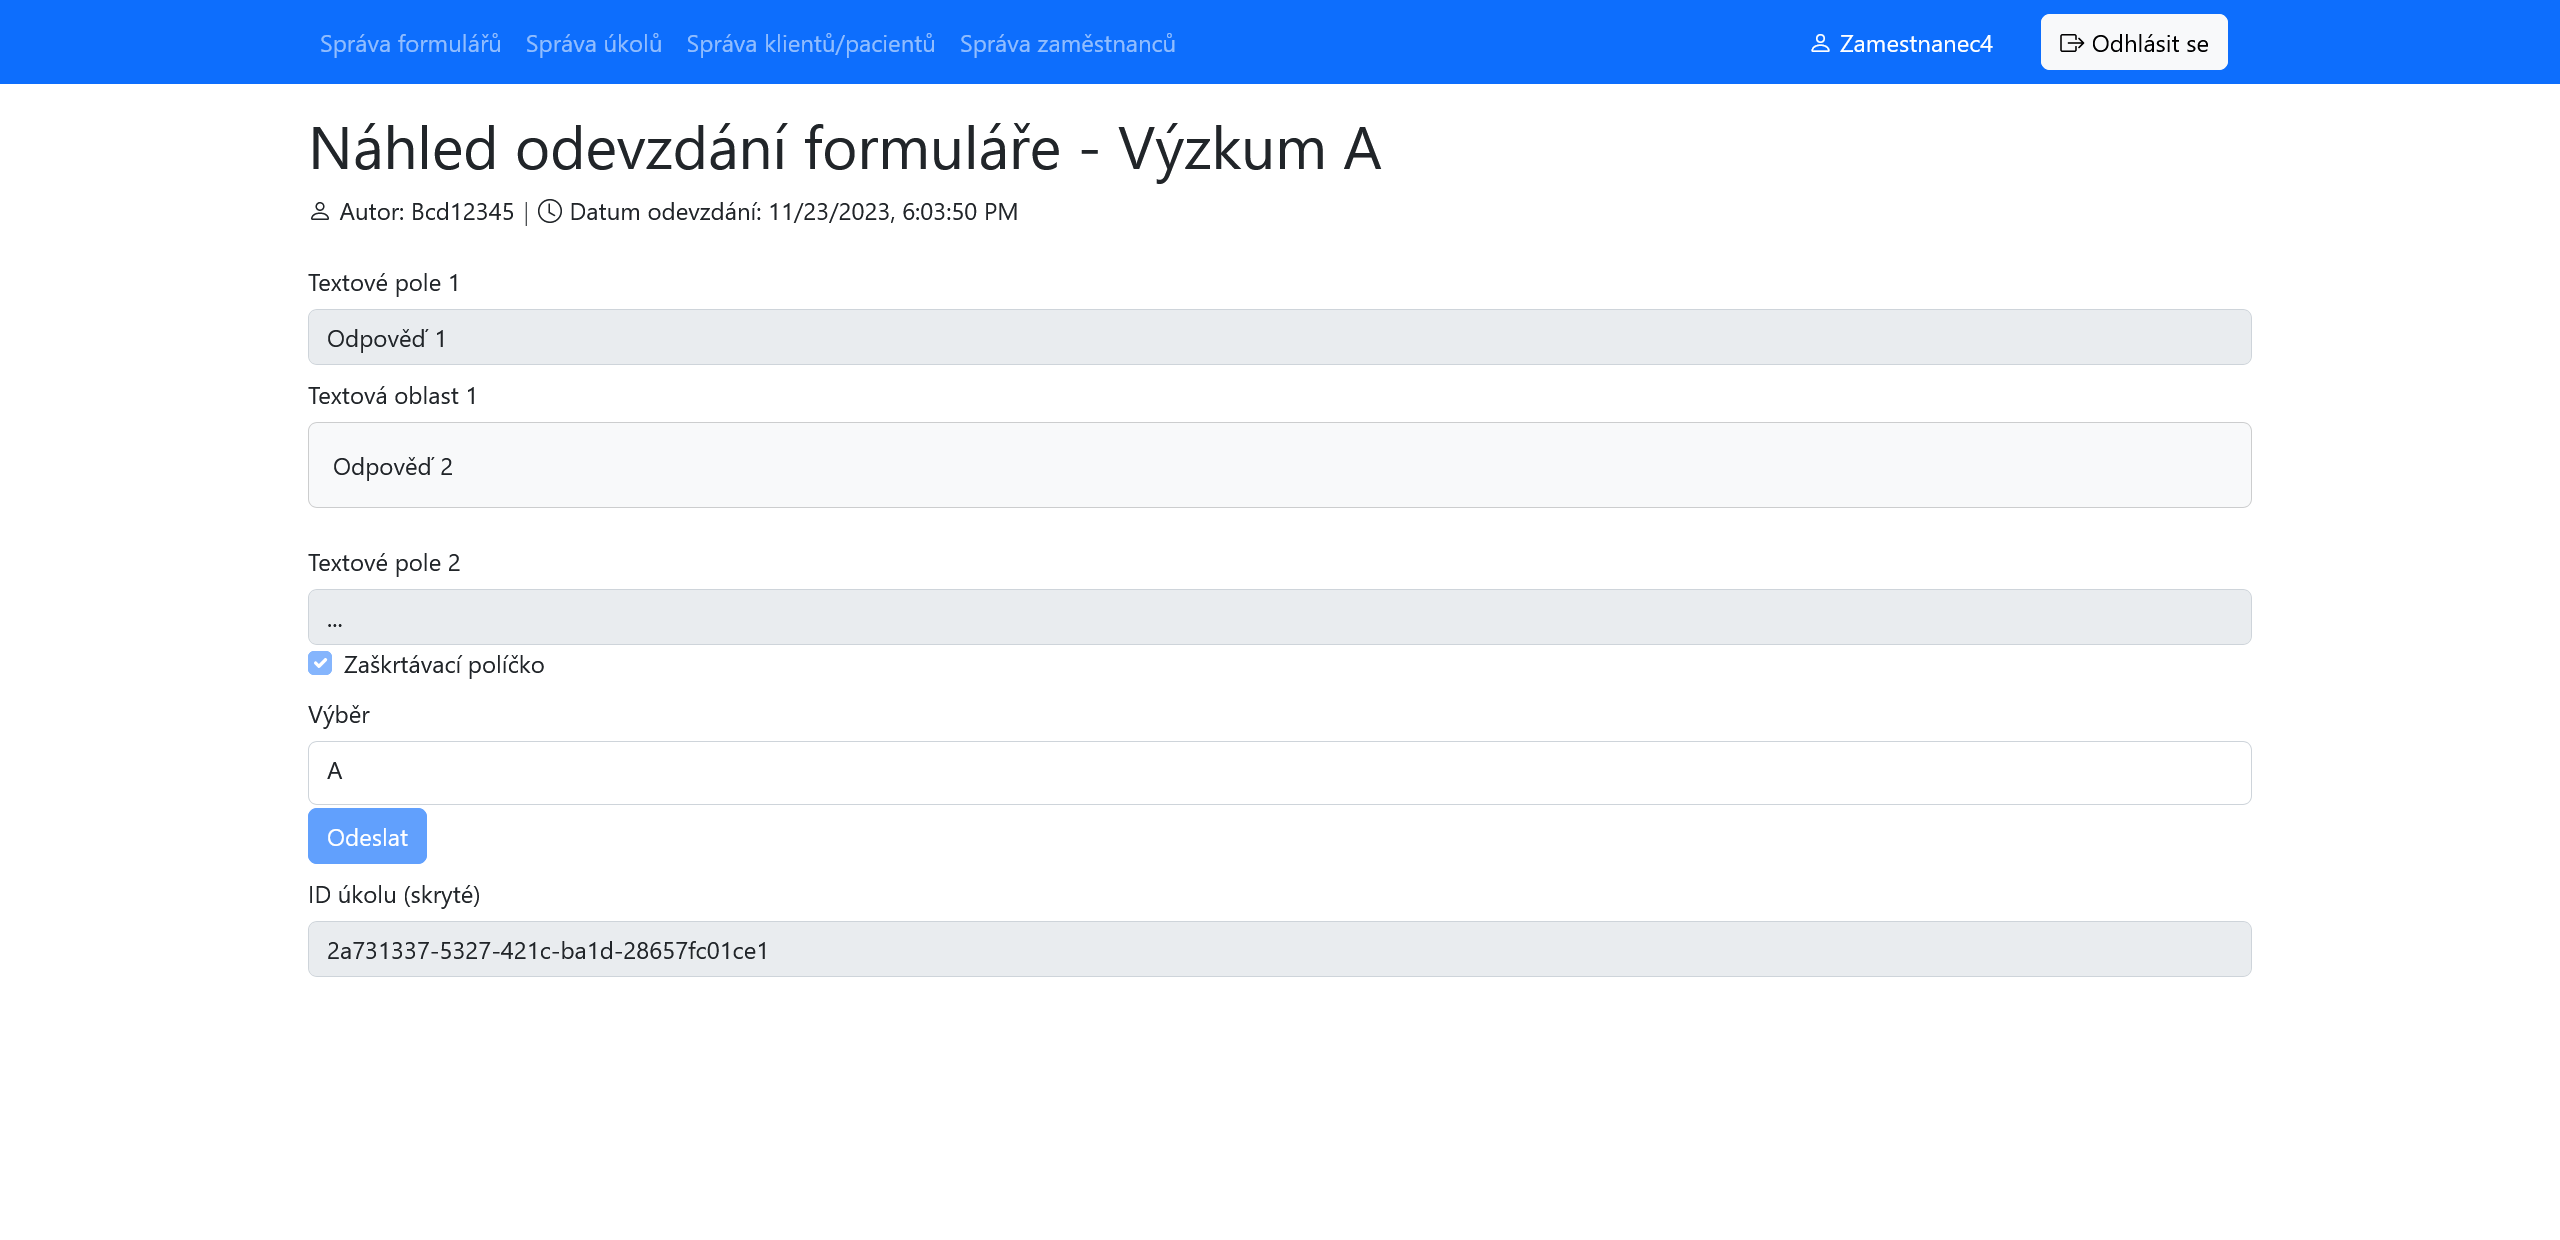
\includegraphics[width=\textwidth]{../img/screenshots/nahled-odevzdani-zamestnanec}
    \caption{Náhled na jednotlivé odevzdání formuláře}\label{fig:nahled-odevzdani-zamestnanec-screenshot}
\end{figure}

Můžeme také zobrazit všechna odevzdání formuláře formou tabulky pomocí tlačítka \uv{Zobrazit všechna odevzdání} v sekci \uv{Správa formulářů} (Obr.~\ref{fig:sprava-formularu-screenshot}).
Tato stránka obsahuje seznam všech odevzdání formuláře (Obr.~\ref{fig:nahled-vsechna-odevzdani-zamestnanec-screenshot}), které lze řadit, filtrovat a následně i exportovat do souboru.
Stránka také umožňuje vytvořit základní vizualizace sesbíraných dat, které lze zobrazit stisknutím tlačítka \uv{Vizualizovat frekvence hodnot} (Obr.~\ref{fig:nahled-vsechna-odevzdani-vizualizace-zamestnanec-screenshot}).
Pokročilejší analýzy a vizualizace dat je možno provádět specializovaným softwarem, který je schopen zpracovat exportovaná data.

\begin{figure}[H]
    \centering
    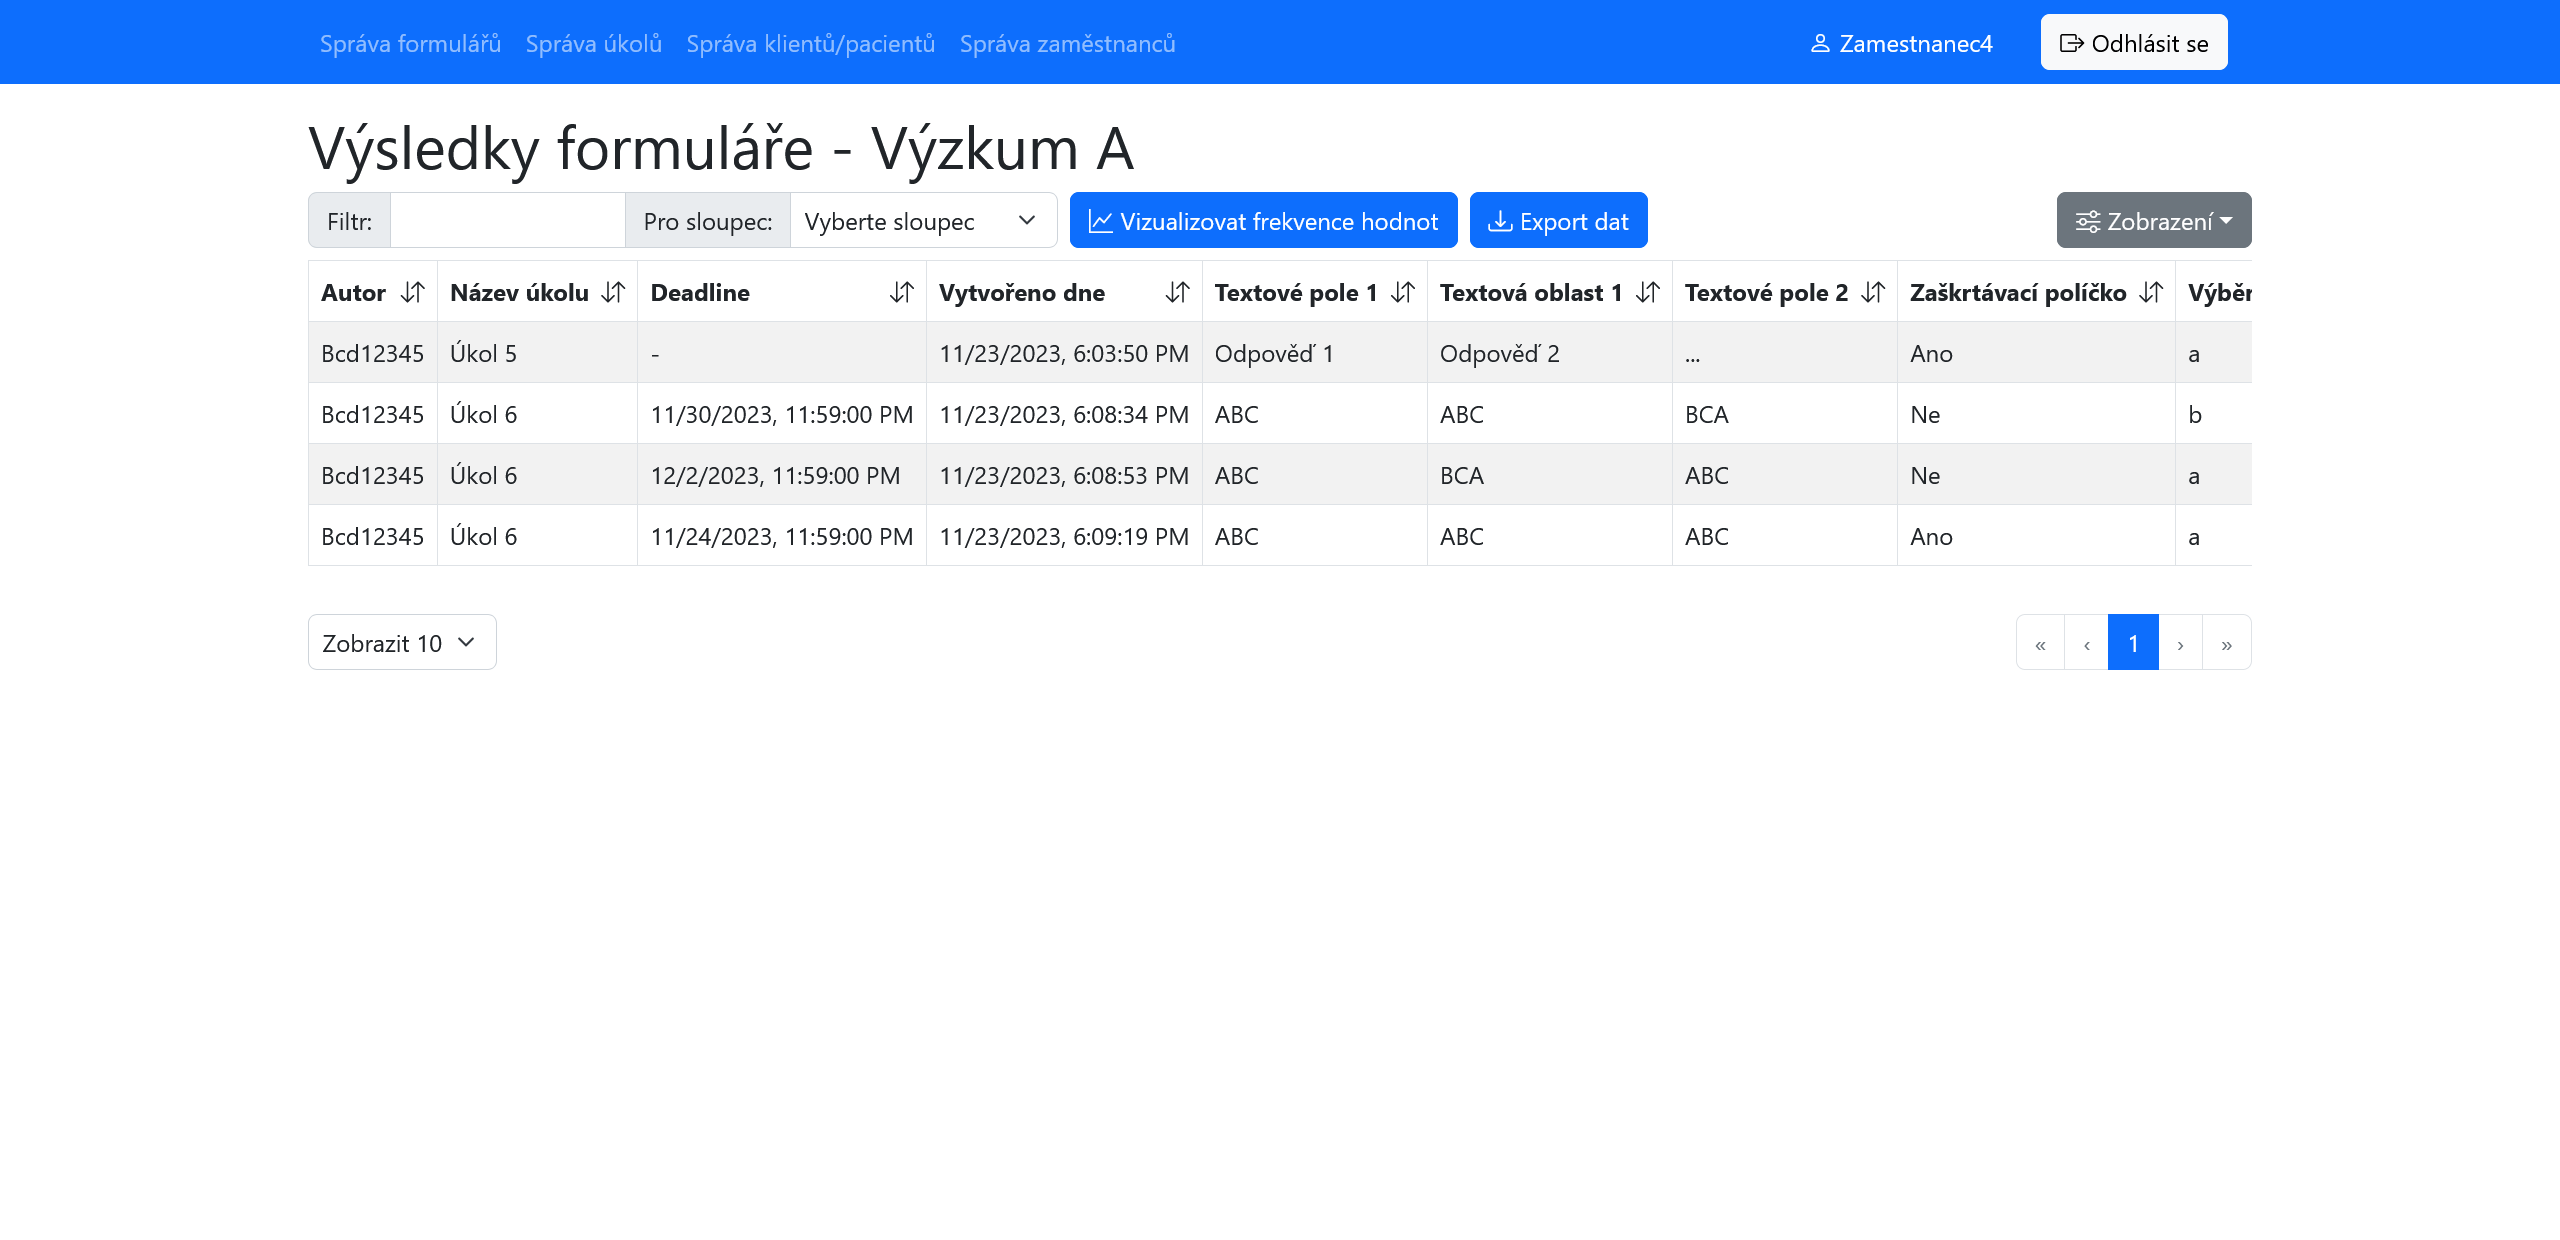
\includegraphics[width=\textwidth]{../img/screenshots/vysledky-formulare}
    \caption{Náhled na všechna odevzdání formuláře}\label{fig:nahled-vsechna-odevzdani-zamestnanec-screenshot}
\end{figure}

\begin{figure}[H]
    \centering
    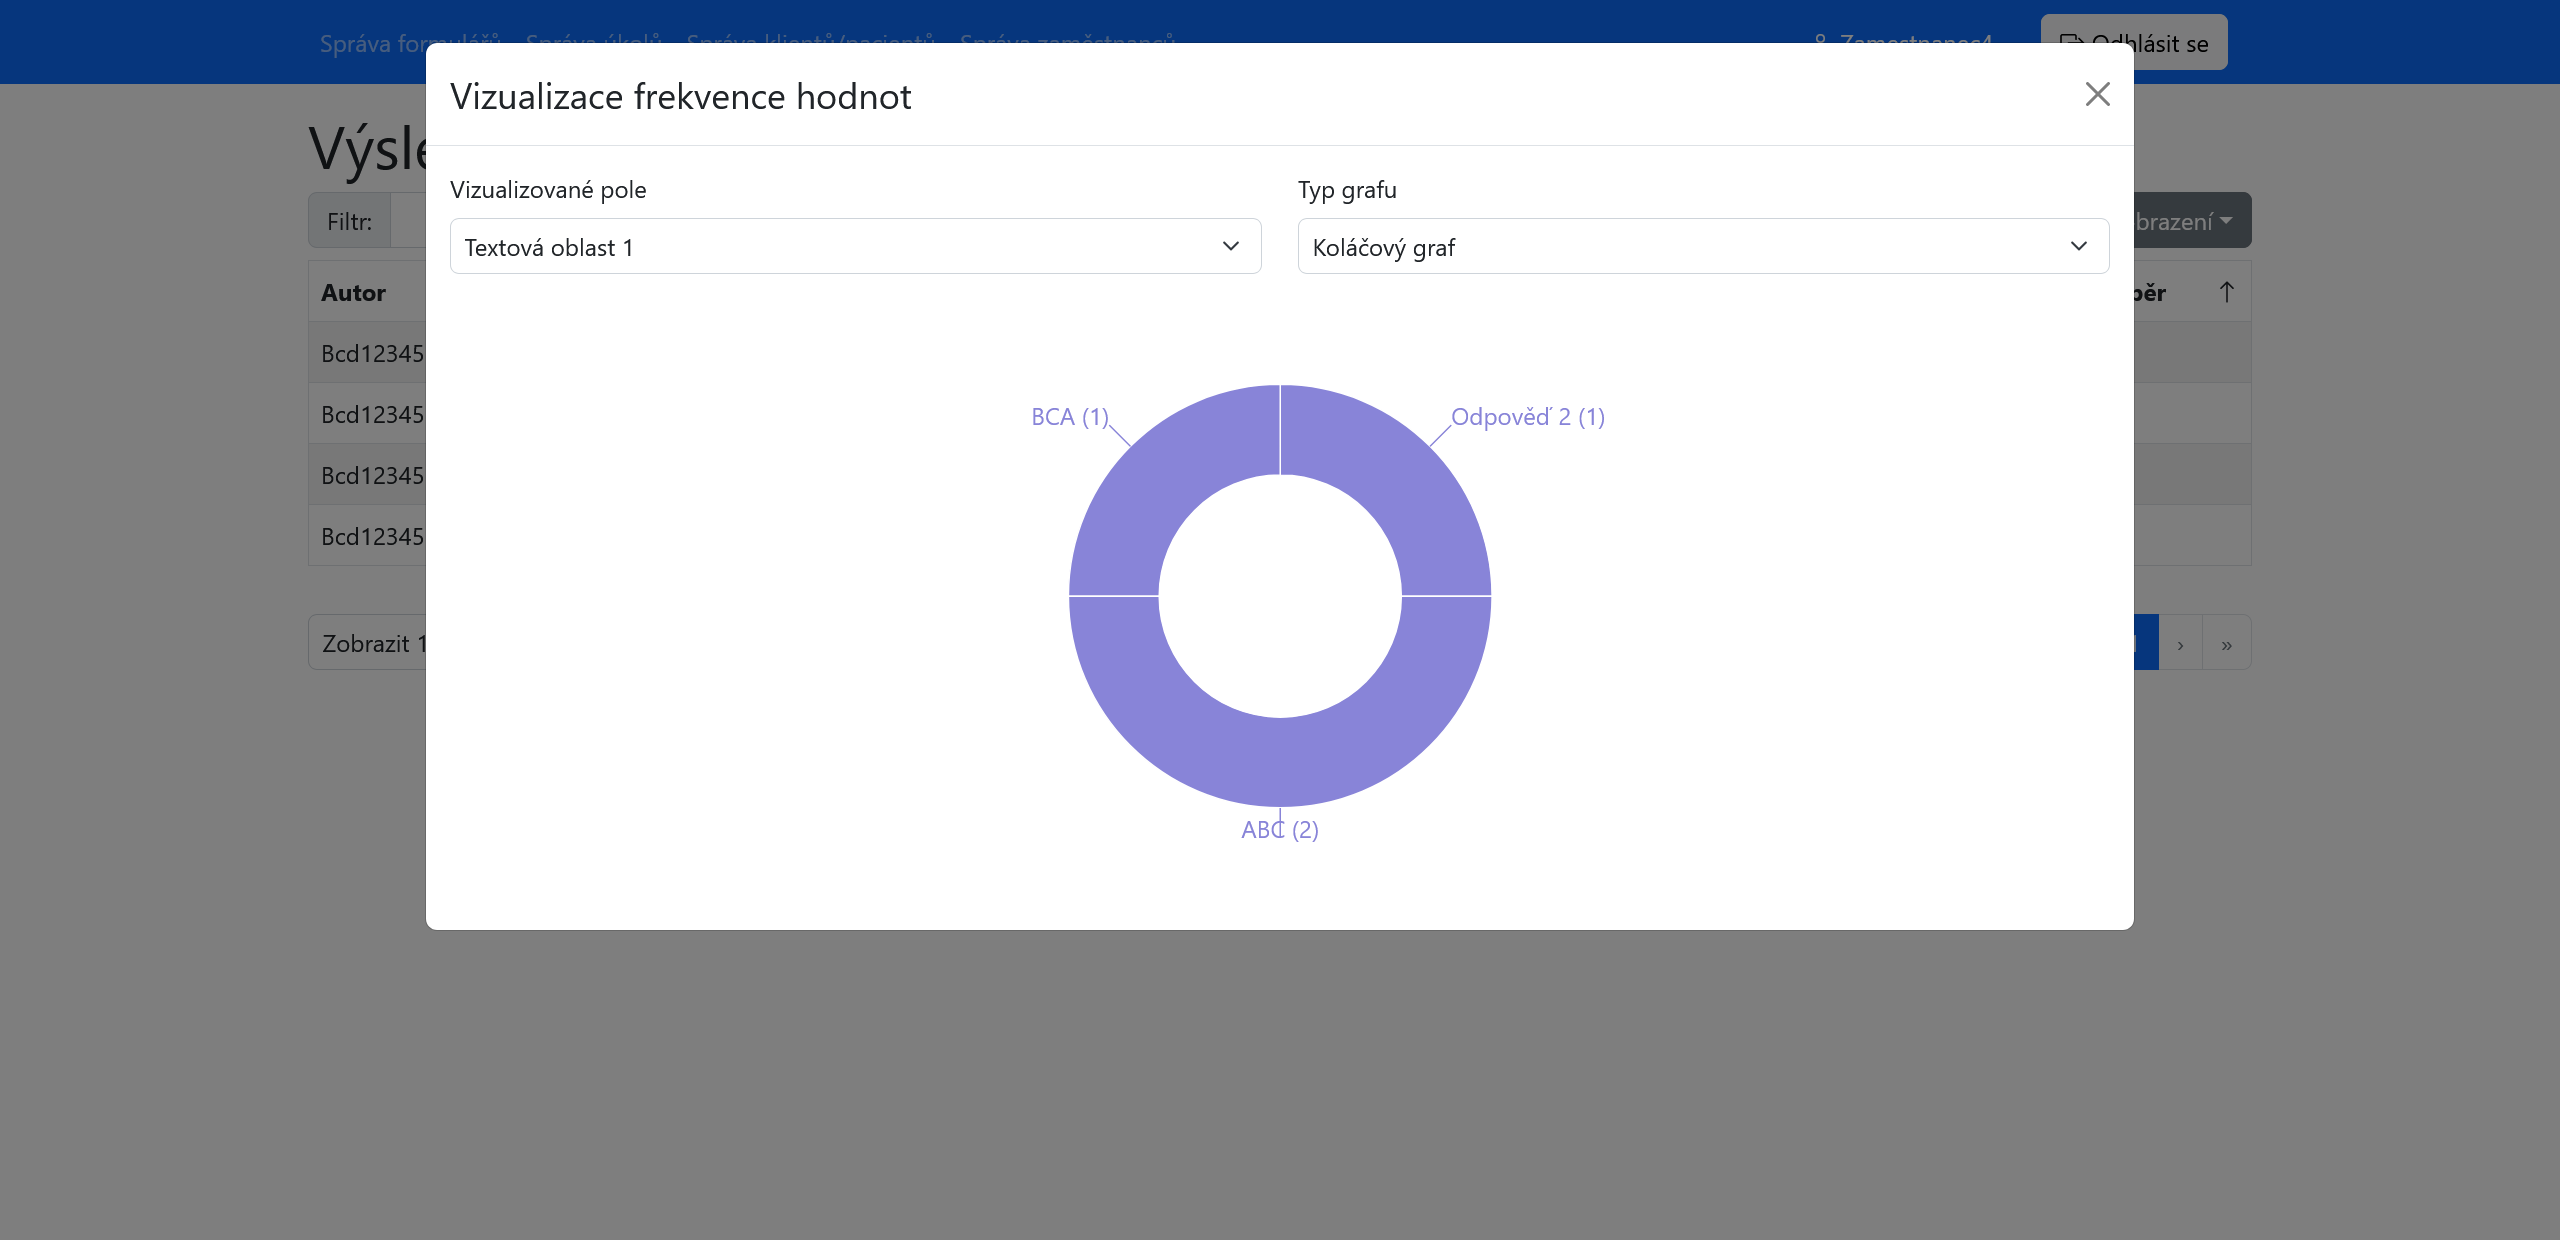
\includegraphics[width=\textwidth]{../img/screenshots/vysledky-formulare-vizualizace}
    \caption{Vizualizace odevzdání formuláře}\label{fig:nahled-vsechna-odevzdani-vizualizace-zamestnanec-screenshot}
\end{figure}

\subsection{Správa účtů}\label{subsec:sprava-uctu}

Zaměstnanec může tvořit účty pro další zaměstnance.
Pokud má zaměstnanec roli \uv{Správce dotazníků}, tak může tvořit účty pro další zaměstnance s rolí \uv{Správce dotazníků} nebo \uv{Zadavatel dotazníků}.
Pokud má zaměstnanec roli \uv{Zadavatel dotazníků}, tak může tvořit účty pro další zaměstnance s rolí \uv{Zadavatel dotazníků}.
Pohled zaměstnance s rolí \uv{Správce dotazníků} je zobrazen na obrázku~\ref{fig:sprava-zamestnancu-screenshot}.

\begin{figure}[H]
    \centering
    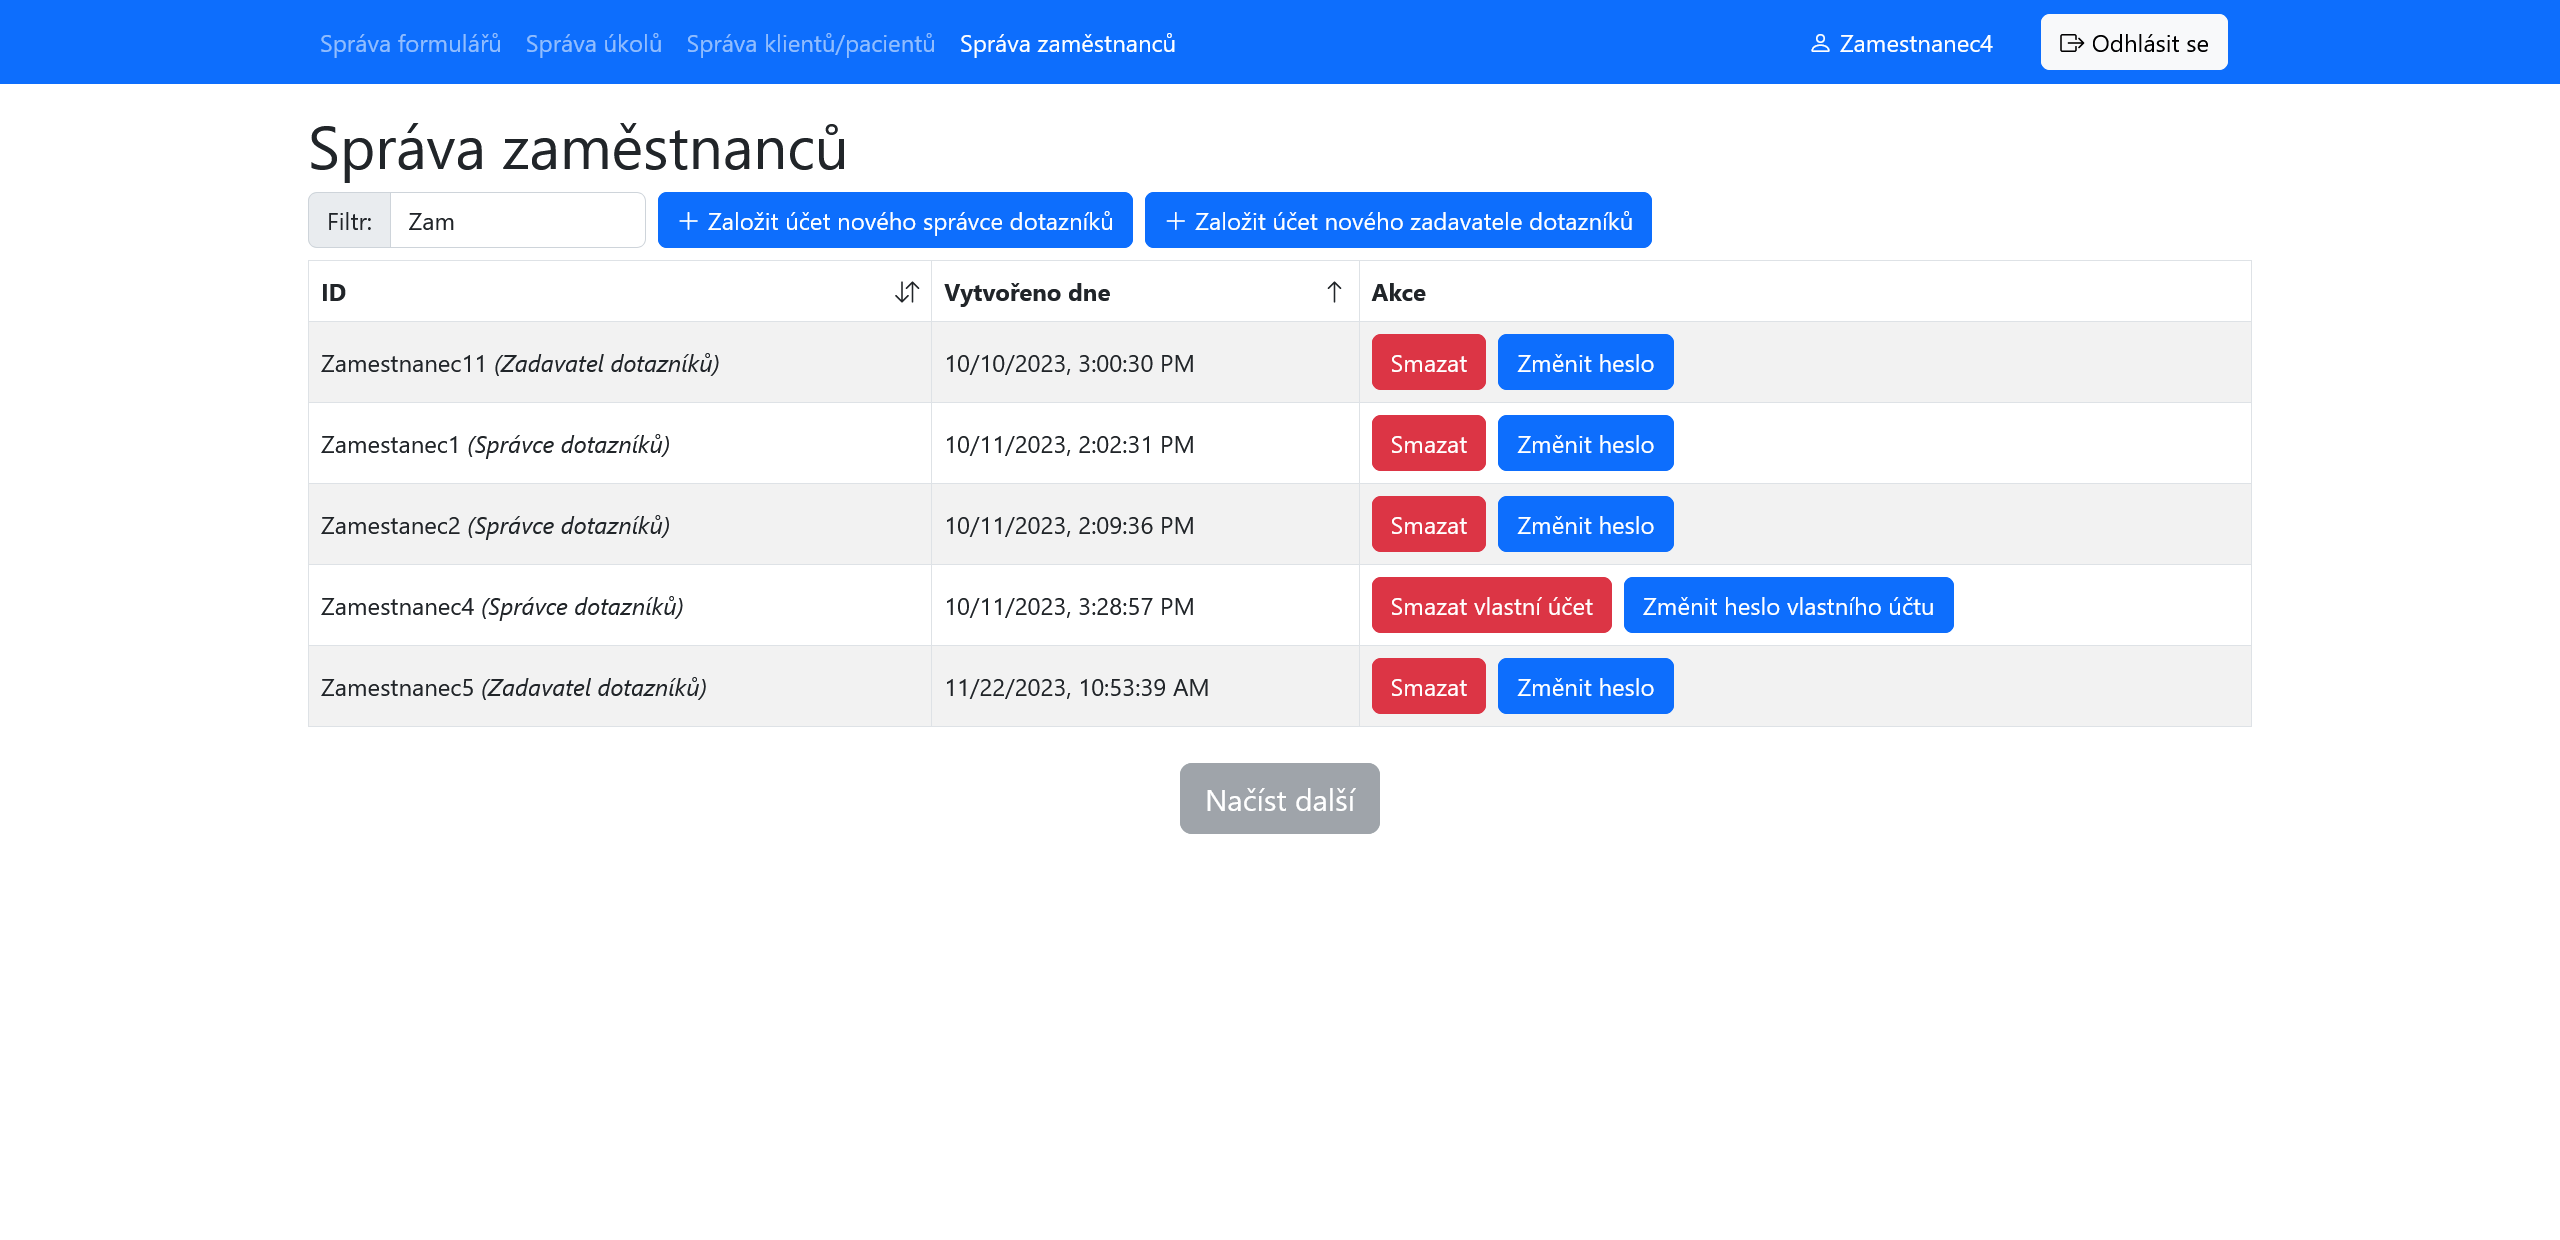
\includegraphics[width=\textwidth]{../img/screenshots/sprava-zamestnancu}
    \caption{Správa zaměstnaneckých účtů}\label{fig:sprava-zamestnancu-screenshot}
\end{figure}

Zaměstnanec si může zobrazit detail svého účtu (Obr.~\ref{fig:zmena-hesla-zamestnanec}) kliknutím na své ID v pravém horním rohu aplikace.
V detailu účtu může zaměstnanec změnit své heslo.

\begin{figure}[H]
    \centering
    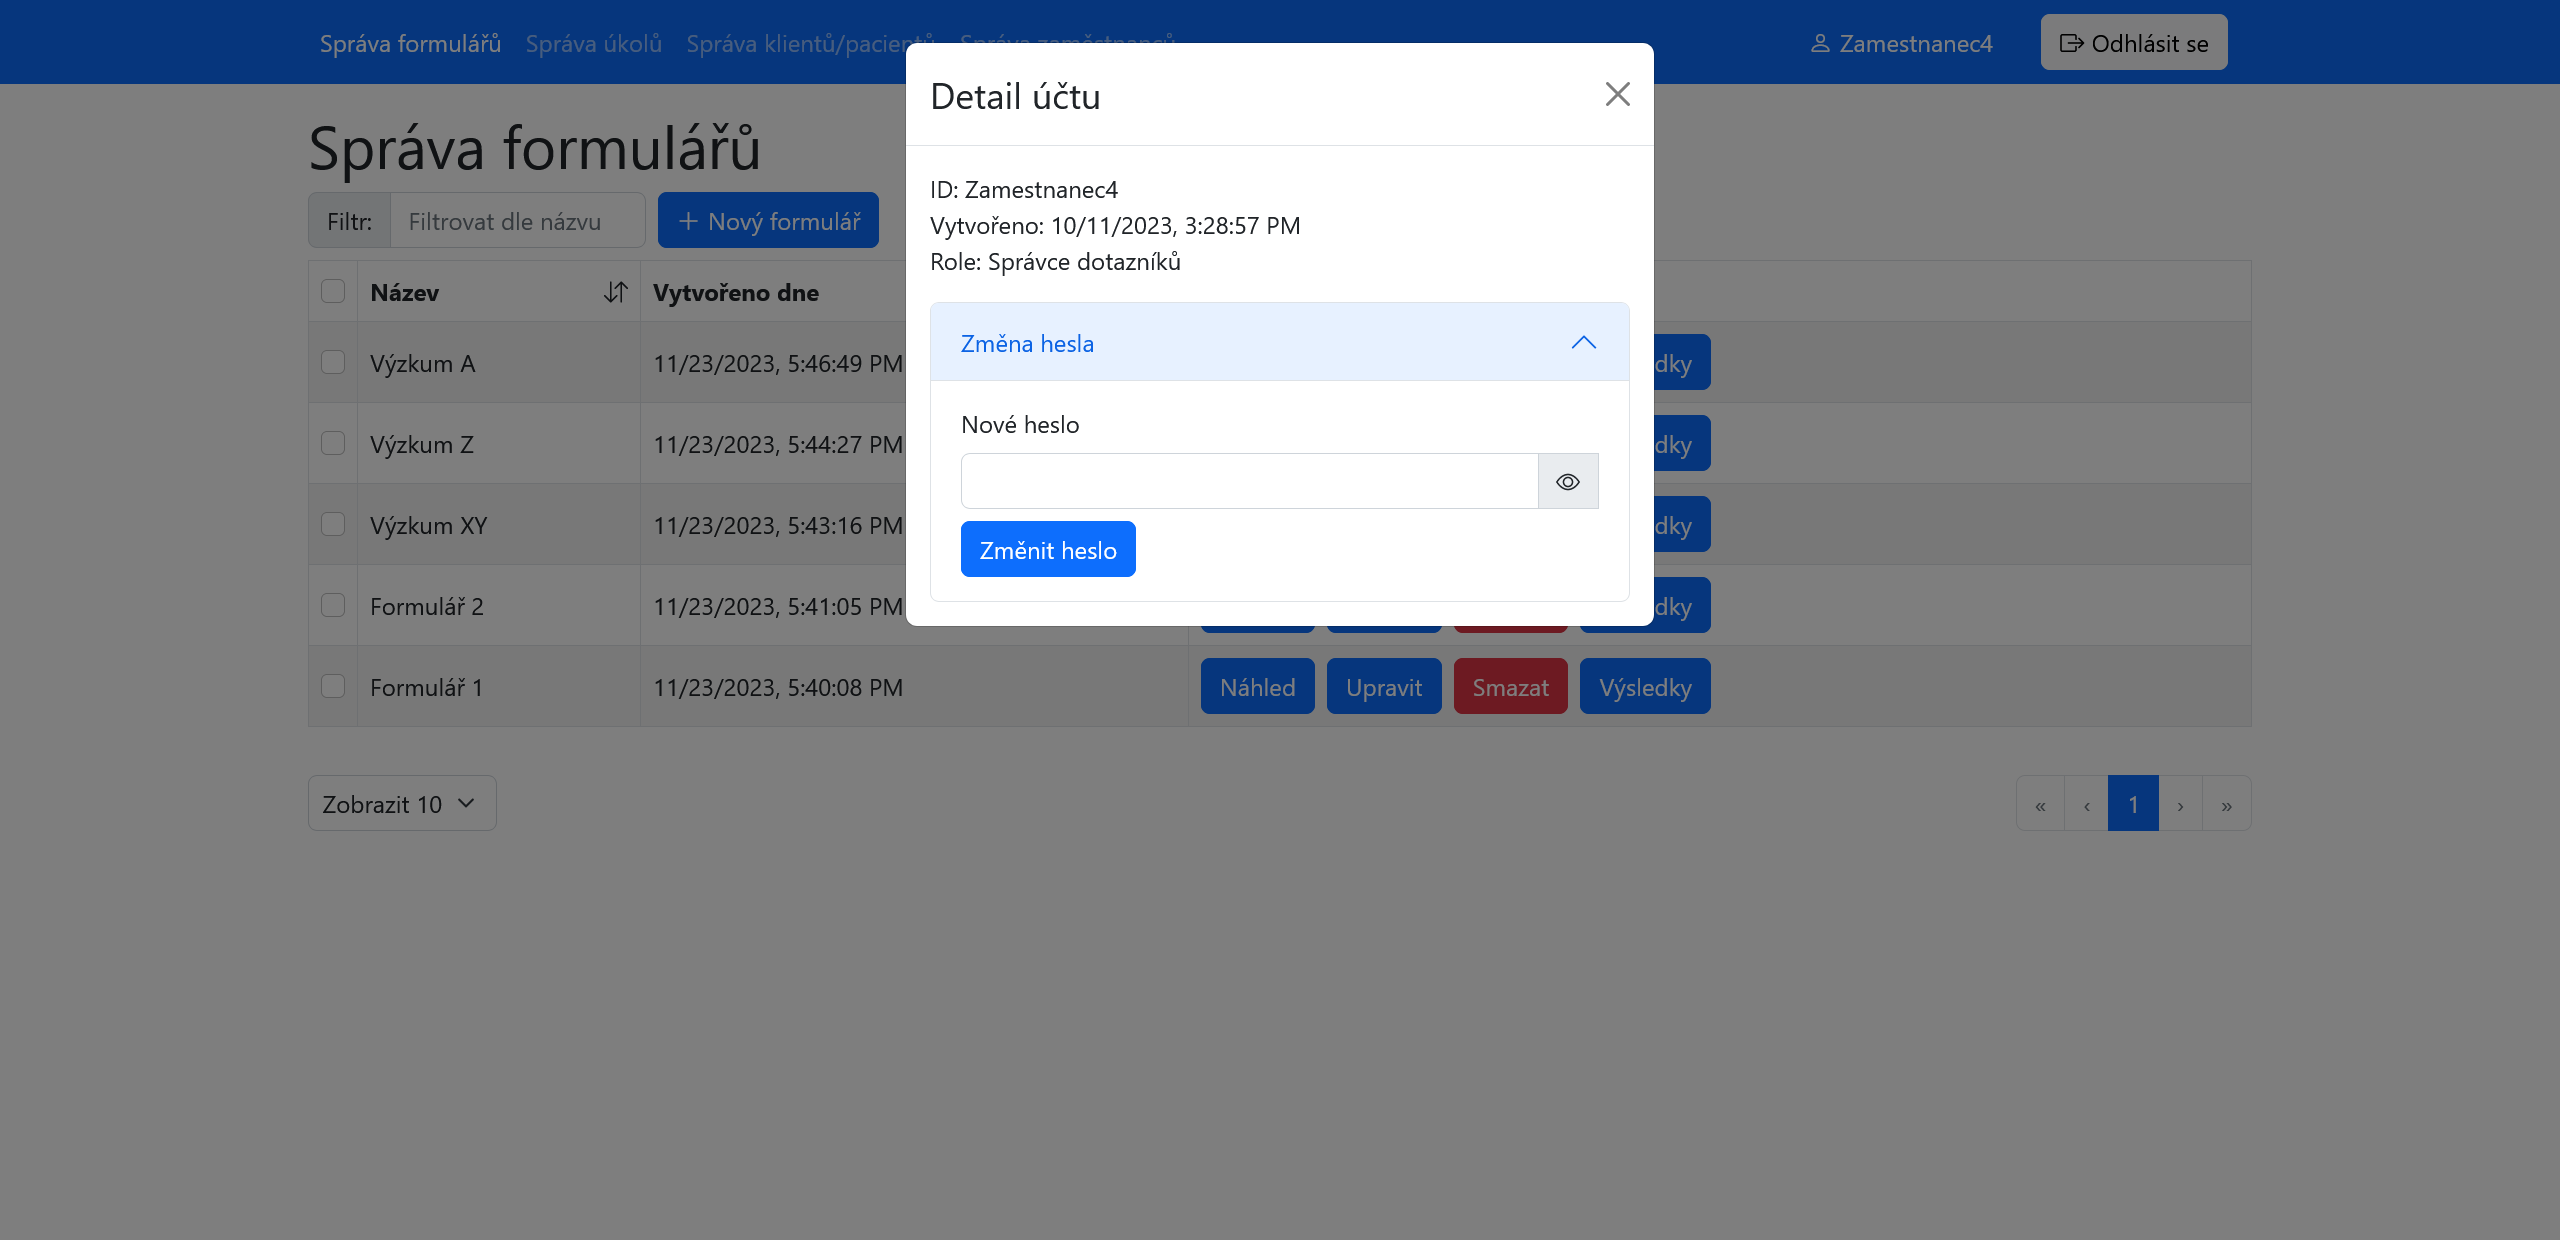
\includegraphics[width=\textwidth]{../img/screenshots/zmena-hesla-zamestnanec}
    \caption{Změna hesla vlastního účtu}\label{fig:zmena-hesla-zamestnanec}
\end{figure}


\section{Užívání aplikace z pohledu plnitele}\label{sec:uzivani-aplikace-z-pohledu-plnitele}

Nyní popišme proces z pohledu plnitele.
Jsou zde popsány veškeré funkce, které byly identifikovány jako požadavky na funkcionalitu dostupnou plniteli v kapitole o analýze požadavků~\ref{ch:analyza-pozadavku}.

Předpokládáme, že plnitel má již vytvořený účet a přihlásil se do aplikace, jak je popsáno v sekci~\ref{sec:prihlaseni}, která se věnuje přihlášení a tvorbě účtu.
Po přihlášení se plnitel dostane na přehled úkolů (Obr.~\ref{fig:prehled-ukolu-uzivatel-screenshot}).
Tato stránka zobrazuje všechny úkoly, které byly plniteli zadány.
Plnitel může úkol splnit stisknutím tlačítka \uv{Splnit}, čímž se dostane na stránku obsahující formulář k vyplnění (Obr.~\ref{fig:vyplneni-formulare-uzivatel-screenshot}).
Plnitel může v průběhu vyplňování formuláře stisknout tlačítko \uv{Uložit koncept}, čímž se formulář uloží do systému, ale neodešle se.
Při návratu na tuto stránku je uložený stav automaticky znovu načten.

\begin{figure}[H]
    \centering
    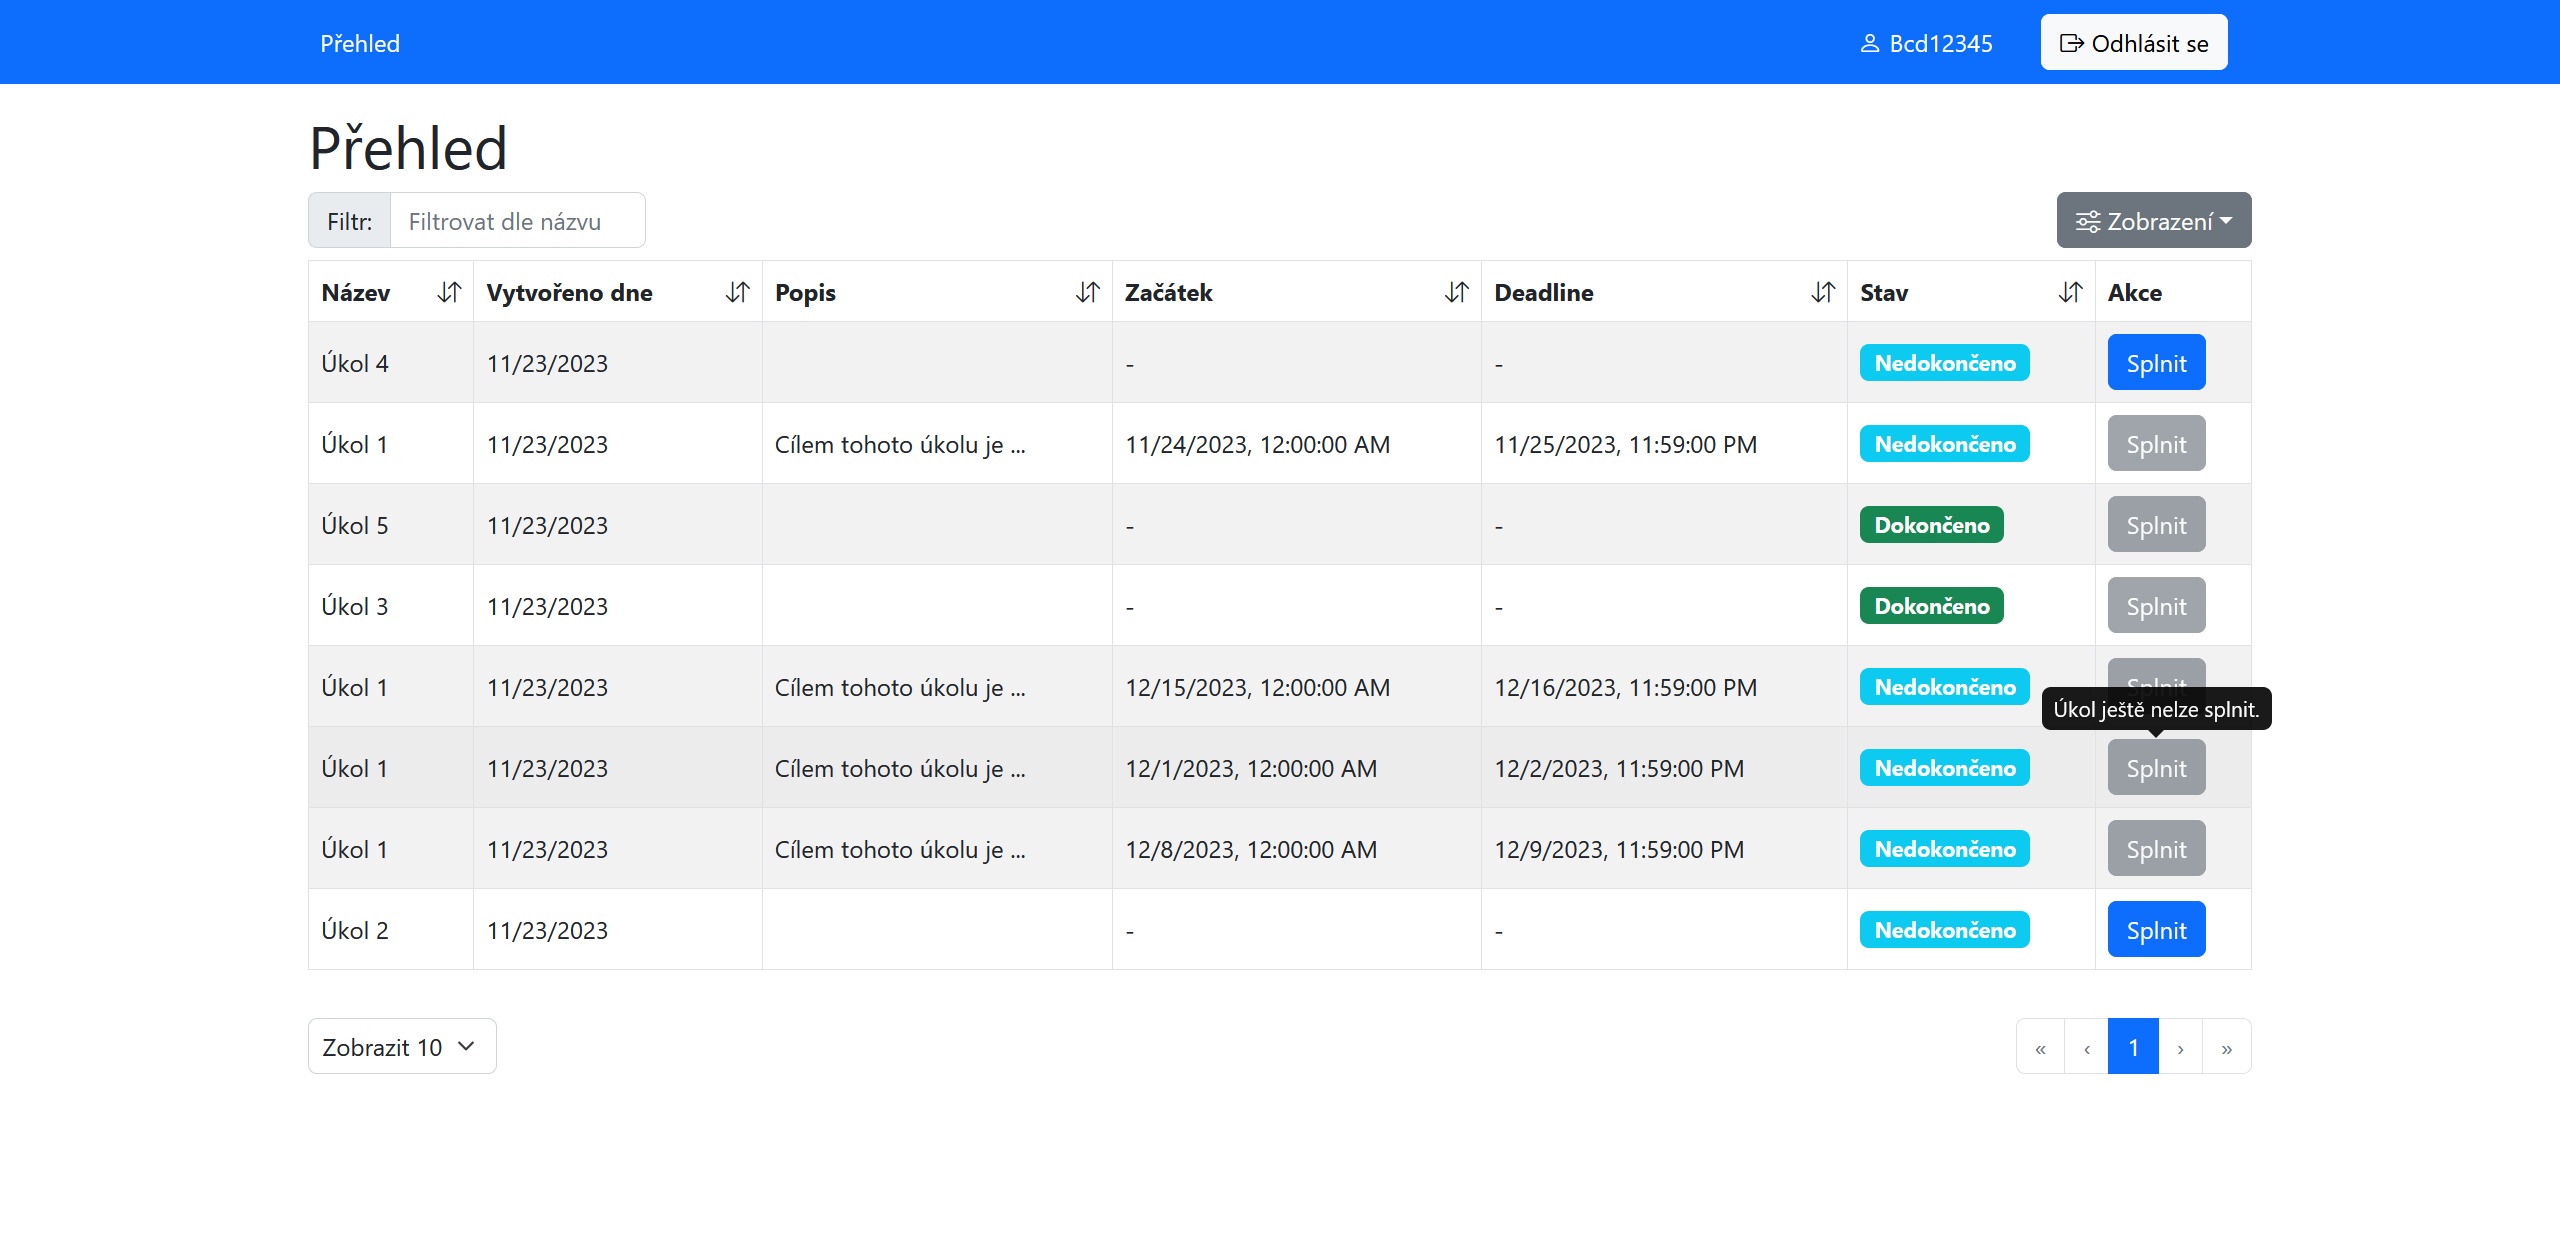
\includegraphics[width=\textwidth]{../img/screenshots/prehled-uzivatel}
    \caption{Přehled úkolů uživatele}\label{fig:prehled-ukolu-uzivatel-screenshot}
\end{figure}

\begin{figure}[H]
    \centering
    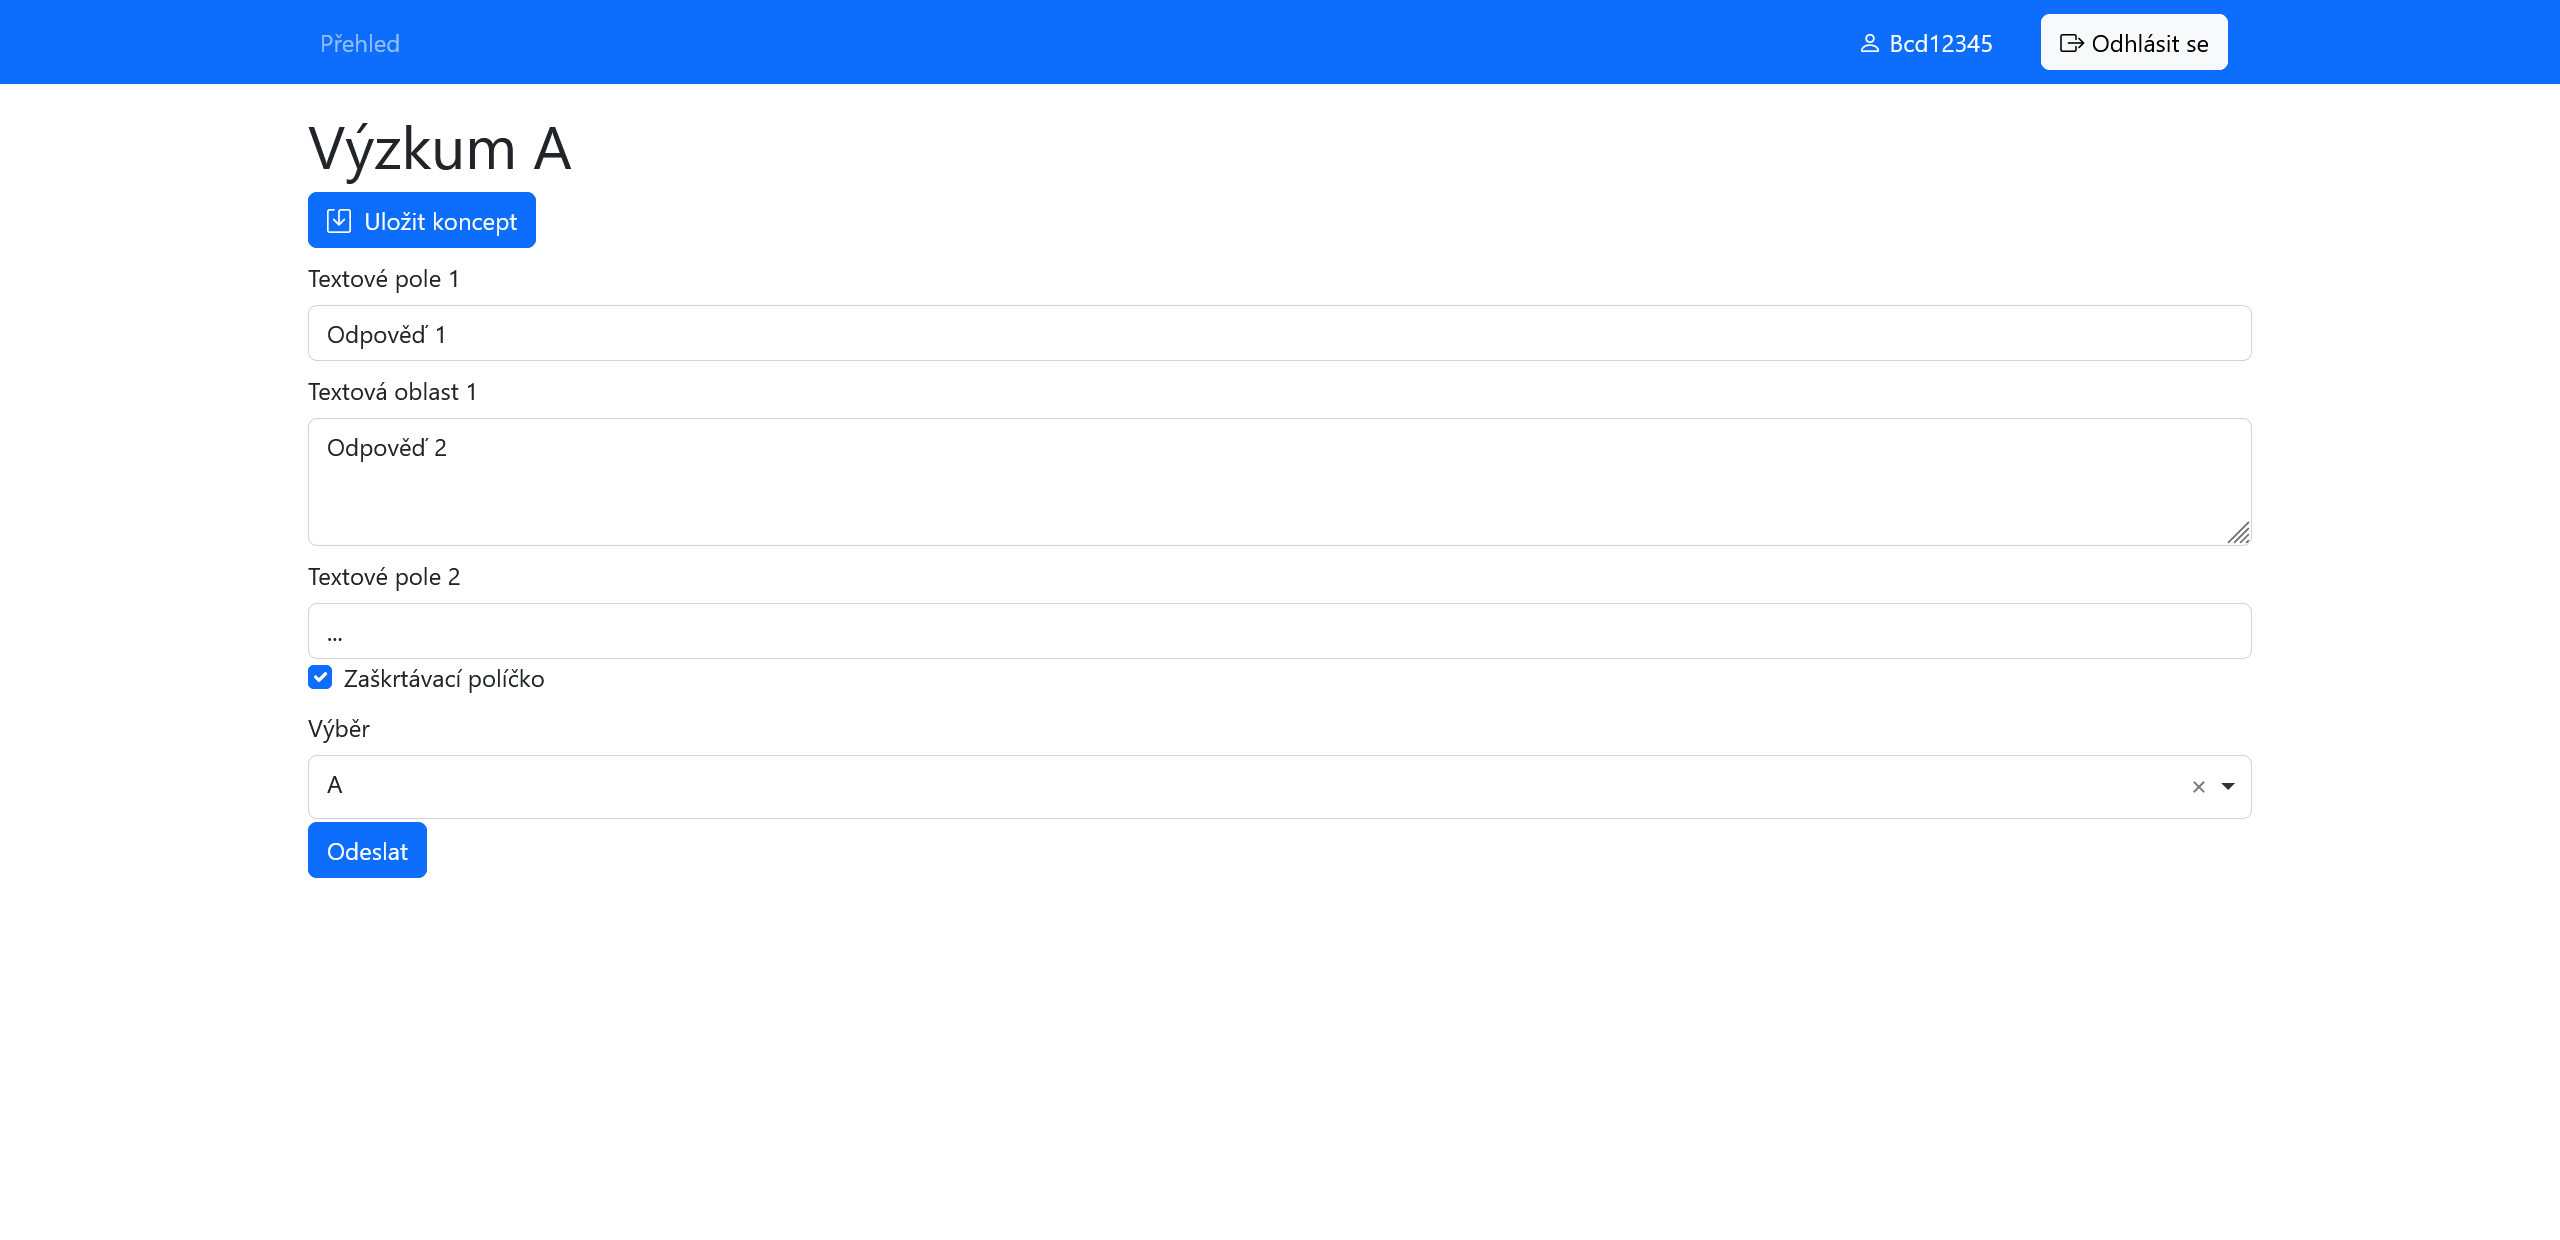
\includegraphics[width=\textwidth]{../img/screenshots/vyplneni-formulare-uzivatel}
    \caption{Vyplnění formuláře plnitelem}\label{fig:vyplneni-formulare-uzivatel-screenshot}
\end{figure}

Uživatel si může zobrazit detail svého účtu (Obr.~\ref{fig:zmena-hesla-uzivatel}) kliknutím na své ID v pravém horním rohu aplikace.
V okně detailu účtu může zaměstnanec změnit své heslo.
Pro změnu hesla je nutno zadat nové heslo a stisknout tlačítko \uv{Změnit heslo}.
Heslo musí obsahovat alespoň jedno velké písmeno, alespoň jedno malé písmeno a alespoň jedno číslo.
Pro manuální kontrolu hesla je možno zobrazit obsah hesla stisknutím tlačítka se symbolem oka.

\begin{figure}[H]
    \centering
    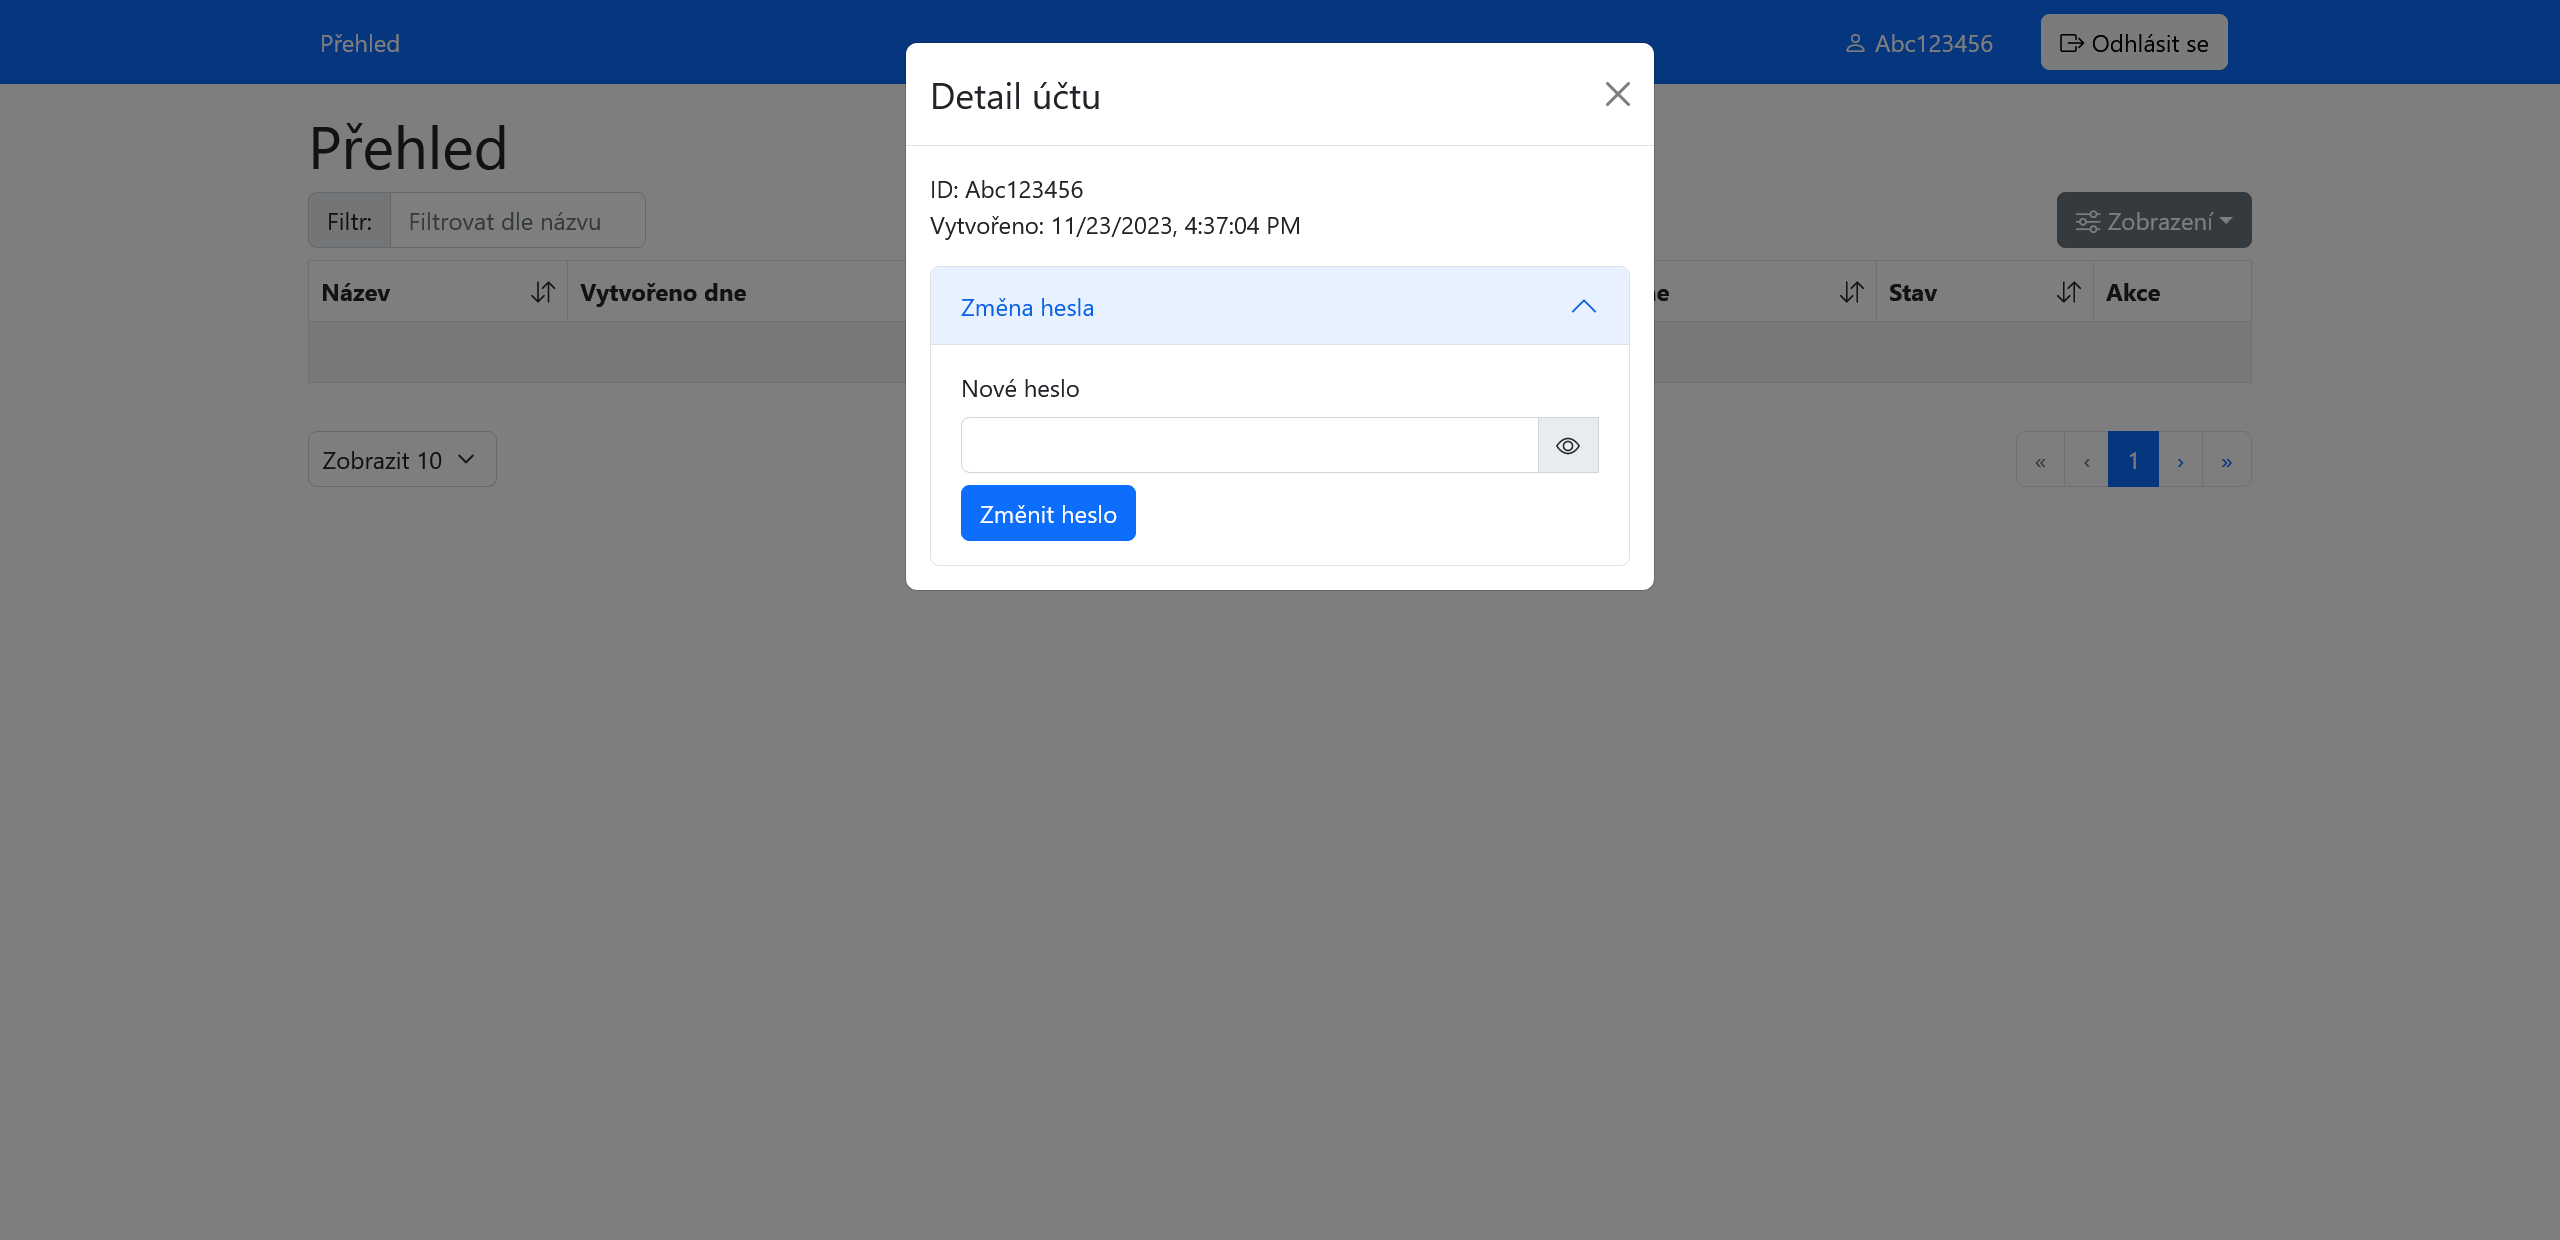
\includegraphics[width=\textwidth]{../img/screenshots/zmena-hesla-uzivatel}
    \caption{Změna hesla vlastního účtu}\label{fig:zmena-hesla-uzivatel}
\end{figure}
